\documentclass[11pt]{article}

% ---------- packages ----------
\usepackage[margin=1in]{geometry}
\usepackage{amsmath,amssymb,amsthm}
\usepackage{graphicx}
\graphicspath{{figs/}}
\usepackage{booktabs}
\usepackage{multirow}
\usepackage{array}
\usepackage{xcolor}
\usepackage{algorithm}
\usepackage{algpseudocode}
\usepackage[numbers,sort&compress]{natbib}
\usepackage[colorlinks=true,linkcolor=blue,citecolor=teal,urlcolor=magenta]{hyperref}
\usepackage{enumitem}
\usepackage{bm}
\usepackage{pifont}

\newtheorem{theorem}{Theorem}
\newtheorem{proposition}{Proposition}
\newtheorem{lemma}{Lemma}
\newtheorem{definition}{Definition}
\newtheorem{remark}{Remark}

\newcommand{\dW}{\Delta W}
\newcommand{\R}{\mathbb{R}}
\newcommand{\trace}{\operatorname{tr}}
\newcommand{\rank}{\operatorname{rank}}
\newcommand{\sign}{\operatorname{sign}}
\newcommand{\diag}{\operatorname{diag}}
\newcommand{\argmin}{\operatorname*{arg\,min}}
\newcommand{\argmax}{\operatorname*{arg\,max}}
\newcommand{\otties}{\textsc{OT-TIES}}
\newcommand{\svdties}{\textsc{SVD-TIES}}

\title{\textbf{OT-TIES: Optimal-Transport Subspaces for\\
Interference-Resolved Merging of Low-Rank Adapters}}

\author{
Hilmi Nur Ardian\\
\texttt{master.ardian@gmail.com}
}
\date{June 2026}

\begin{document}
\maketitle

\begin{abstract}
Merging a bank of task-specialized Low-Rank Adapters (LoRAs) into a single multi-task model without
retraining is an attractive route to compute-frugal model reuse. The strongest existing methods
(KnOTS, Core Space, GeoMerge) succeed by two coupled ingredients: (i) they build a \emph{shared
subspace} in which the per-task updates are expressed, and (ii) inside that subspace they
\emph{resolve interference} (sign election, magnitude trimming) rather than naively averaging.
The subspace, however, is invariably chosen by a singular value decomposition (SVD) of the stacked
task updates -- an algebraic, geometry-agnostic choice. In this paper we ask whether
\emph{optimal transport} (OT) yields a better shared subspace. We make three contributions.
First, we give a careful negative result: merging LoRA adapters by an OT \emph{average}
(a Wasserstein barycenter of their singular-direction distributions) plateaus at the
simple-averaging floor regardless of target rank or scaling, because averaging blurs rather than
resolves sign interference. Second, we introduce \otties{}, which keeps the TIES interference-resolution
operator but replaces the SVD-chosen merge subspace by the leading subspace of a \emph{Wasserstein
barycenter} of the tasks' rank-$r$ direction distributions. On the standard $8$-task CLIP ViT-B/32
LoRA benchmark, with an \emph{identical} TIES combiner, the OT-chosen subspace beats the SVD-chosen
subspace at every scaling we test ($+0.7$ to $+1.9$ normalized-accuracy points), lifting the merged
model from the $\sim\!0.64$ naive floor to $0.708$. Third, we show a structural capability that the
rank-fixed baselines cannot offer: because \otties{} (and a Gromov--Wasserstein variant) operate on
the full update $\dW=BA$ rather than a fixed-rank quotient, they natively merge a
\emph{heterogeneous-rank} adapter zoo (ranks $\{4,8,16\}$), losing only $1.0$ point relative to the
homogeneous case -- a setting GeoMerge's fixed-rank quotient and Core Space's shared rank-$r$ basis
cannot enter at all. Every merge runs on CPU in minutes; the entire study was produced on free
Kaggle GPUs used only for evaluation. Code, configurations, and all logs are released.
\end{abstract}

\tableofcontents
\newpage

% =====================================================================
\section{Introduction}
\label{sec:intro}

Parameter-efficient fine-tuning (PEFT), and Low-Rank Adaptation (LoRA) in particular
\citep{hu2022lora}, has made it cheap to specialize a single pre-trained backbone into many
task experts: one freezes the backbone $W_0$ and learns, per task $t$, a low-rank update
$\dW_t = B_t A_t$ with $B_t \in \R^{m\times r}$, $A_t \in \R^{r\times n}$ and $r \ll \min(m,n)$.
The resulting adapters are tiny (a few megabytes), composable, and shared in the thousands on public
hubs. This abundance raises a natural question: given a \emph{bank} of task-specialized LoRAs for the
same backbone, can we \emph{merge} them into a single model that performs all tasks well, without any
further training and without access to task data?

Model merging \citep{wortsman2022soups,ilharco2023task,yadav2023ties,li2023deepfusion} answers
``sometimes.'' The naive answer -- average the weights, or sum the task vectors
$\sum_t \dW_t$ -- degrades badly as the number of tasks grows, because independently trained updates
\emph{interfere}: they overlap in parameter space, disagree in sign, and differ wildly in magnitude
\citep{yadav2023ties}. The merging literature has converged on two complementary fixes.
\textbf{Interference resolution} (TIES \citep{yadav2023ties}, DARE \citep{yu2024dare}) trims small
entries, elects a per-coordinate sign by majority, and averages only the agreeing tasks.
\textbf{Subspace alignment} (KnOTS \citep{stoica2024knots}, Core Space \citep{panariello2025corespace},
GeoMerge \citep{dasilva2026geomerge}, EpiMer \citep{lu2026epimer}) first projects every task into a
common low-dimensional basis -- typically obtained from an SVD of the stacked updates -- so that
interference resolution operates on aligned coordinates. The state of the art for LoRA merging marries
the two: KnOTS performs TIES \emph{inside} an SVD-aligned space, and Core Space / GeoMerge refine the
choice of basis and the averaging geometry.

A striking commonality runs through these strong methods: \emph{the shared subspace is always chosen
by linear algebra}. KnOTS concatenates the task factors and takes their SVD; Core Space builds a
common alignment basis by SVD; GeoMerge averages on a fixed-rank Riemannian quotient
$(\mathrm{St}\times\mathrm{SPD}\times\mathrm{St})/O(r)$ whose charts again come from SVD. None of them
asks whether the \emph{geometry of how the tasks' directions correspond to one another} should inform
the basis. This is precisely the question optimal transport is built to answer: OT computes a coupling
between two distributions of mass that minimizes a ground cost, and its barycenter computes the
distribution that is jointly closest, in transport distance, to a family of distributions
\citep{villani2009ot,peyre2019computational,agueh2011barycenters}. If we view a LoRA update as a small
distribution over its singular directions, OT offers a principled, geometry-aware way to align and
combine tasks.

OT is, surprisingly, almost absent from the merging literature. A recent survey of $200{+}$ merging
methods finds only a handful that use transport at all, and the one explicit OT-merging paper, OTMF
\citep{pan2025otmf}, transports \emph{activation} distributions to learn masks (a data-dependent,
full-model procedure), not the weight-space, data-free, low-rank merge we study. The classical OT model
fusion of \citet{singh2020fusion} aligns \emph{neurons} across full $d\times d$ layers -- expensive and
unrelated to the low-rank structure of LoRA. The lane ``merge LoRA adapters by optimal transport in the
rank-$r$ subspace'' is essentially empty.

\paragraph{This paper.}
We investigate whether OT yields a better merge subspace than SVD, with a deliberately controlled
comparison, and we report both a negative and a positive result.

\begin{enumerate}[leftmargin=1.4em,itemsep=2pt]
\item \textbf{A clean negative result (Section~\ref{sec:method-averaging}, \ref{sec:results-averaging}).}
The most ``natural'' OT merge -- represent each task as a distribution over its rank-$r$ singular
directions and take their \emph{Wasserstein barycenter} -- does \emph{not} beat naive averaging. Across
target ranks $\{16,32,64,128\}$ and scalings, OT-barycenter and OT-alignment both plateau at the
simple-average floor ($\approx 0.62$ normalized accuracy), \emph{below} tuned task arithmetic.
The reason is structural and we make it precise: a transport barycenter is still an \emph{average}, so it
blurs and cancels conflicting directions; it does not perform the sign election that interference
resolution requires.

\item \textbf{A positive, controlled result (Section~\ref{sec:method-otties}, \ref{sec:results-otties}).}
We introduce \otties{}: keep the TIES interference-resolution operator, but choose the shared subspace
as the leading left-singular subspace of the \emph{Wasserstein barycenter} of the task direction
distributions, rather than the SVD of the stacked factors (the KnOTS-style choice). Holding the TIES
combiner \emph{identical}, the OT-chosen subspace beats the SVD-chosen subspace \emph{at every scaling
tested} on the $8$-task ViT-B/32 LoRA benchmark ($+0.7$ to $+1.9$ points), with a peak of
$0.708$ normalized accuracy versus $0.687$ for the SVD control and $0.64$ for the naive floor.
This isolates the contribution of the \emph{geometry of the subspace choice} from the contribution of
interference resolution.

\item \textbf{A structural capability the baselines lack
(Section~\ref{sec:method-gw}, \ref{sec:results-hetero}).}
Because \otties{} operates on the full update $\dW_t=B_tA_t$ rather than a fixed-rank manifold, and
because we also provide a Gromov--Wasserstein (GW) variant that couples tasks by their \emph{intra-task}
geometry, our method natively merges a \emph{heterogeneous-rank} adapter zoo (mixed ranks
$\{4,8,16\}$). It loses only $1.0$ point relative to the homogeneous-rank case -- in a regime where
GeoMerge's fixed-rank quotient and Core Space's shared rank-$r$ basis cannot operate at all without
ad-hoc padding.
\end{enumerate}

\begin{figure}[t]
\centering
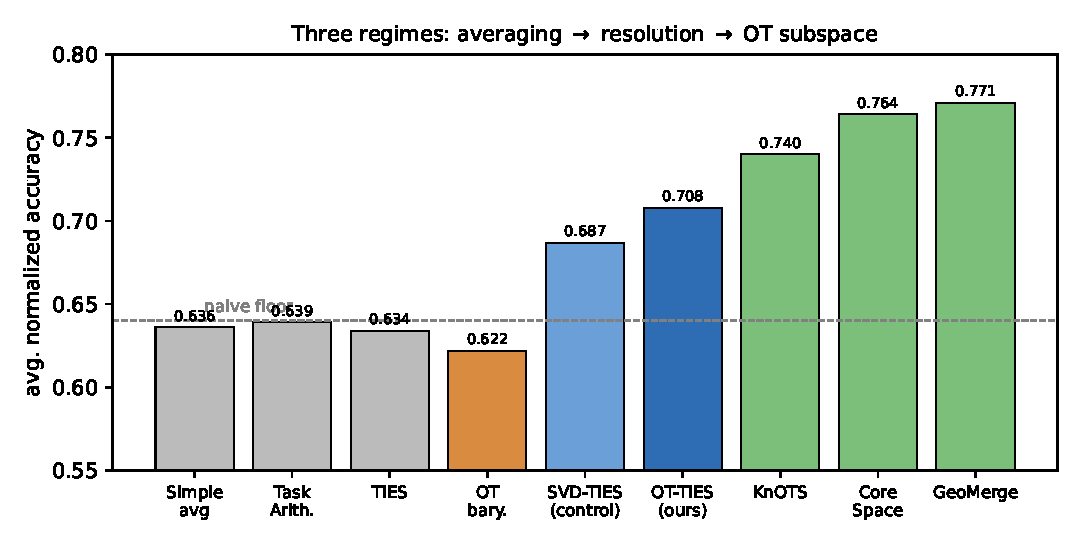
\includegraphics[width=0.92\textwidth]{regimes.pdf}
\caption{The three regimes we identify on the $8$-task ViT-B/32 LoRA benchmark. Naive merges (gray) and
the OT \emph{average} (orange) cluster at the $\sim\!0.64$ floor. Interference resolution in a shared
subspace lifts the merge off the floor (\svdties{} control, light blue), and choosing that subspace by
optimal transport rather than SVD adds a further, consistent gain (\otties{}, dark blue). The published
advanced methods (green) are the bar to beat; the gap to them is largely attributable to our simplified
combiner, not to the OT subspace (Section~\ref{sec:analysis}).}
\label{fig:regimes}
\end{figure}

\paragraph{Compute-frugality as a first-class goal.}
Every merge in this paper is a sequence of small ($r\times r$ to $k\times k$, $r\le 16$, $k\le 128$)
linear-algebra operations and runs on a CPU in minutes for the full ViT-B/32 model; no GPU is needed for
the merge itself, only for evaluation. The complete study -- reproducing five baseline configurations,
two failed OT-averaging families, the \otties{} ablation grid, and the heterogeneous-rank experiment --
was carried out entirely on the free tier of Kaggle (30 GPU-hours/week, T4/P100), using the GPU solely to
evaluate merged models. We view this not merely as convenience but as part of the contribution: a
geometry-principled merge that is cheap by construction lowers the barrier for low-resource and
Global-South laboratories to reuse the growing public stock of adapters. We release the full codebase,
all configurations, and every run log.

\begin{table}[t]
\centering
\caption{Summary of findings (8-task ViT-B/32 LoRA; average normalized accuracy). The contribution is
the controlled OT-over-SVD subspace advantage and the heterogeneous-rank capability, both at
compute-frugal CPU cost.}
\label{tab:summary}
\small
\begin{tabular}{lll}
\toprule
Finding & Evidence & Section \\
\midrule
OT \emph{averaging} does not beat the naive floor & $0.61$--$0.63$ at all ranks/scales & \ref{sec:results-averaging} \\
Interference resolution lifts off the floor & \svdties{} $0.687$, \otties{} $0.708$ vs $0.64$ & \ref{sec:results-otties} \\
OT subspace $>$ SVD subspace, identical combiner & $+0.7$ to $+1.9$ pts, every $\lambda$ & \ref{sec:results-otties} \\
Heterogeneous-rank merge (baselines cannot) & mixed $\{4,8,16\}$ at $0.698$ ($-1.0$ pt) & \ref{sec:results-hetero} \\
Compute-frugal by construction & $264$--$359$\,s CPU, full model & \ref{sec:results-compute} \\
\bottomrule
\end{tabular}
\end{table}

% =====================================================================
\section{Related Work}
\label{sec:related}

\subsection{Model merging and task arithmetic}
Weight averaging of fine-tuned models was popularized by Model Soups \citep{wortsman2022soups}, which
showed that averaging models fine-tuned with different hyperparameters can improve accuracy at no
inference cost. Task Arithmetic \citep{ilharco2023task} reframed merging in terms of \emph{task
vectors} $\tau_t = \theta_t - \theta_0$, observing that $\theta_0 + \lambda \sum_t \tau_t$ yields a
serviceable multi-task model and that negating a task vector ``forgets'' a task. Git Re-Basin
\citep{ainsworth2023rebasin} aligns models modulo permutation symmetries before averaging, an early
signal that \emph{alignment} matters. A comprehensive taxonomy appears in the deep model fusion survey
of \citet{li2023deepfusion}.

\subsection{Interference resolution}
TIES-Merging \citep{yadav2023ties} identified three interference modes when summing task vectors --
redundant parameters, sign conflicts, and magnitude disparities -- and resolves them by
(i) \emph{trimming} all but the top-magnitude entries of each task vector, (ii) electing a per-parameter
sign by the sign of the aggregate, and (iii) averaging only the tasks that agree with the elected sign.
DARE \citep{yu2024dare} shows that delta parameters are highly redundant and can be randomly dropped and
rescaled before merging. These operators are the empirical backbone of strong merges; our \otties{}
re-uses the TIES operator unchanged and varies only the subspace it acts in.

\subsection{Subspace / SVD alignment for LoRA merging}
LoRA updates are explicitly low rank, which makes the choice of a \emph{shared} subspace both natural
and consequential. KnOTS \citep{stoica2024knots} aligns the per-task updates in a common space obtained
by SVD of the concatenated factors, then applies TIES; it substantially improves over space-agnostic
TIES. Core Space \citep{panariello2025corespace} merges low-rank adaptations inside a common alignment
basis, preserving low-rank efficiency while improving accuracy, and reports state-of-the-art results on
vision and language LoRA benchmarks. Decouple-and-Orthogonalize \citep{zheng2025decouple} addresses the
large magnitude disparities specific to LoRA factors. IterIS \citep{chen2025iteris} refines an alignment
by iterative inference-solving. A parallel line constrains the LoRA subspace \emph{before} or
\emph{during} fine-tuning to reduce later interference: LoRI \citep{zhang2025lori} freezes $A$ as a
random projection and sparsifies $B$ with task masks; \citet{zhang2025unraveling} pre-allocate
orthogonal subspaces; LEGO \citep{zhao2025lego} clusters rank-one components for modular reuse. All of
these obtain the shared basis algebraically (SVD, orthogonality, random projection). We instead obtain
it by optimal transport and compare head-to-head with the SVD choice under an identical combiner.

\subsection{The geometry of merging}
A recent and influential thread recasts merging as averaging on a \emph{manifold}. GeoMerge
\citep{dasilva2026geomerge} formulates merging as a Fr\'echet average under an explicit geometry and,
with a high-rank lift, sets the current state of the art on the $8$-task ViT-B/32 LoRA benchmark
($77.1\%$ normalized accuracy). EpiMer \citep{lu2026epimer} computes a Fr\'echet mean on a Riemannian
manifold restricted to the task-vector subspace using a projected Hessian. On the optimization side,
Stiefel-LoRA \citep{park2025stiefel}, RiemannLoRA \citep{bogachev2025riemannlora}, and Riemannian
preconditioned LoRA \citep{zhang2024riemannian} bring Riemannian geometry to LoRA \emph{training};
AlignGuard-LoRA \citep{das2025alignguard} uses Fisher-guided decomposition to preserve alignment.
These methods share a feature that bounds their applicability: their manifolds are \emph{rank-fixed}
(the quotient $(\mathrm{St}\times\mathrm{SPD}\times\mathrm{St})/O(r)$ and the shared rank-$r$ basis both
require all adapters to have the same rank $r$). Our heterogeneous-rank experiment
(Section~\ref{sec:results-hetero}) targets exactly the regime these methods cannot enter.
Concretely, EpiMer \citep{lu2026epimer} restricts the Fr\'echet mean to the task-vector subspace and
exploits a projected Hessian for curvature, while GeoMerge \citep{dasilva2026geomerge} parameterizes the
merged adapter on the product manifold of left/right Stiefel factors and an SPD core, quotiented by the
$O(r)$ rotation gauge -- a construction that is only well defined when all adapters share the rank $r$
that fixes the Stiefel and SPD dimensions. The Riemannian-\emph{training} line
\citep{zhang2024riemannian,park2025stiefel,bogachev2025riemannlora} likewise pins the rank during
optimization. None of these can accept a bank of adapters with ranks $\{4,8,16\}$ without first padding or
projecting to a common $r$ (which either fabricates or discards signal). Our method needs no such
homogenization because it works on $\dW_t=B_tA_t$ and a fixed ambient dimension $k$.

\subsection{Optimal transport in model merging}
OT is mature in machine learning -- Sinkhorn's entropic regularization \citep{cuturi2013sinkhorn} made
it differentiable and fast; Wasserstein barycenters \citep{agueh2011barycenters} average distributions
geometrically; Gromov--Wasserstein \citep{memoli2011gromov,peyre2016gromov} couples distributions across
\emph{incomparable} spaces; the POT library \citep{flamary2021pot} provides solvers. Yet in merging, OT
is rare. \citet{singh2020fusion} fuse models by transporting \emph{neurons} across full layers -- a
$d\times d$ problem unrelated to low-rank structure. OTMF \citep{pan2025otmf} transports
\emph{activation} distributions to learn fusion masks in a continual setting, requiring data forward
passes. To our knowledge no prior work uses OT to choose the \emph{weight-space, data-free, low-rank}
merge subspace, which is the gap we fill.

\subsection{PEFT, LoRA optimization, and continual adaptation}
A broad literature improves \emph{how} LoRAs are trained and structured, which is complementary to (and
upstream of) merging. On optimization, LoRA-Pro \citep{wang2024lorapro} corrects the gradient geometry of
the low-rank factors, LoRA-GA \citep{wang2024loraga} aligns the initial update with the full-fine-tuning
gradient, and the Riemannian-training family \citep{zhang2024riemannian,park2025stiefel,bogachev2025riemannlora}
optimizes the factors on Stiefel/quotient manifolds to remove the scale/rotation ambiguity intrinsic to
$BA$. On structure and efficiency, Uni-LoRA \citep{li2025unilora} reinterprets many LoRA variants as a
single global subspace projection, LISA \citep{pan2024lisa} replaces low-rank updates with layerwise
importance sampling, LoSiA \citep{wang2025losia} localizes high-rank subnets, and a stronger
mixture-of-LoRA-experts \citep{sun2025moelora} preconditions expert gradients. The
\emph{asymmetry} of the two factors -- $A$ extracts features, $B$ projects them -- was made explicit by
\citet{zhu2024asymmetry}, motivating our use of paired (left\,$\times$\,right) ground costs rather than a
single-factor cost. In continual settings, C-LoRA \citep{zhang2025clora} and the perturb-then-merge
framework of \citet{qiu2025perturbmerge} fold merging into the learning loop. RDP-LoRA
\citep{celebi2026rdplora} and CopRA \citep{zhuang2024copra} use representational geometry and progressive
training respectively to choose where/how to adapt. Our work is orthogonal to all of these: it takes
\emph{already-trained} adapters (of possibly heterogeneous rank) and asks only how best to combine them,
data-free and training-free.

\subsection{Positioning}
In one sentence: prior strong LoRA merges resolve interference inside an \emph{SVD-chosen} shared
subspace; we keep the resolver and replace the subspace by an \emph{OT-chosen} one, and we additionally
remove the rank-homogeneity assumption that the geometric state of the art structurally requires.
Table~\ref{tab:methodcompare} places the main methods on the axes that matter for this paper.

\begin{table}[t]
\centering
\caption{Where the main data-free LoRA-merge methods sit. ``Subspace'' = how the shared basis is chosen;
``Combine'' = averaging vs.\ interference resolution; ``Het.\ rank'' = can it merge adapters of
\emph{different} ranks without padding; ``CPU merge'' = the merge step needs no GPU.}
\label{tab:methodcompare}
\small
\begin{tabular}{lllcc}
\toprule
Method & Subspace & Combine & Het.\ rank & CPU merge \\
\midrule
Task Arithmetic \citep{ilharco2023task} & none (ambient) & scaled sum & \checkmark & \checkmark \\
TIES \citep{yadav2023ties} & none (ambient) & resolution & \checkmark & \checkmark \\
KnOTS \citep{stoica2024knots} & SVD of stacked factors & resolution (TIES) & \checkmark$^\dagger$ & \checkmark \\
Core Space \citep{panariello2025corespace} & SVD alignment basis & resolution & \ding{55} (rank-$r$) & partly \\
GeoMerge \citep{dasilva2026geomerge} & fixed-rank quotient & Fr\'echet \emph{average} & \ding{55} (rank-$r$) & \ding{55} (Riem.\ loop) \\
\midrule
\textbf{OT-TIES (ours)} & \textbf{OT barycenter} & resolution (TIES) & \checkmark & \checkmark \\
\textbf{GW (ours)} & GW (intra-task) & resolution & \checkmark & \checkmark \\
\bottomrule
\end{tabular}
\\[2pt]
{\footnotesize $^\dagger$ KnOTS's stacked-SVD basis admits mixed column counts in principle but is not
evaluated in that regime; the geometric methods (Core/GeoMerge) are rank-fixed by construction.}
\end{table}

% =====================================================================
\section{Background and Problem Setup}
\label{sec:background}

\begin{table}[h]
\centering
\caption{Notation.}
\label{tab:notation}
\small
\begin{tabular}{ll}
\toprule
Symbol & Meaning \\
\midrule
$W_0\in\R^{m\times n}$ & frozen backbone weight at a layer \\
$A_t\in\R^{r_t\times n},\,B_t\in\R^{m\times r_t}$ & LoRA down/up factors of task $t$ \\
$s_t=\alpha_t/r_t$ & LoRA scaling of task $t$ \\
$\dW_t=s_tB_tA_t$ & task-$t$ update; $\dW^\star$ the merged update \\
$U_t,\Sigma_t,V_t$ & thin SVD factors of $\dW_t$ (Stiefel, diagonal, Stiefel) \\
$\mu_t=\sum_k p_{t,k}\delta_{(u_{t,k},v_{t,k})}$ & task-$t$ direction distribution, $p_{t,k}\propto\sigma_{t,k}$ \\
$T$ & number of tasks/adapters; $r$ common rank when homogeneous \\
$k$ & shared-subspace dimension ($k\le \sum_t r_t$) \\
$\kappa$ & TIES keep fraction; $\lambda$ scale; $\varepsilon$ Sinkhorn reg. \\
$C\in\R^{r_i\times r_j}$ & ground cost; $P\in\Pi(\bm p,\bm q)$ transport plan \\
$\nu$ & Wasserstein barycenter of $\{\mu_t\}$; $U$ its leading subspace \\
$\mathrm{NA}$ & average normalized accuracy (Eq.~\eqref{eq:na}) \\
\bottomrule
\end{tabular}
\end{table}

\subsection{LoRA updates and the merging problem}
Fix a backbone with frozen weight $W_0\in\R^{m\times n}$ at a given layer. A LoRA adapter for task $t$
adds
\begin{equation}
\dW_t \;=\; s_t\, B_t A_t, \qquad B_t\in\R^{m\times r_t},\; A_t\in\R^{r_t\times n},\;
s_t = \frac{\alpha_t}{r_t},
\label{eq:lora}
\end{equation}
where $s_t$ is the LoRA scaling ($\alpha_t$ is the configured \texttt{lora\_alpha}). Given $T$ adapters
$\{(A_t,B_t,s_t)\}_{t=1}^T$ for the \emph{same} backbone, a layer-wise merge produces a single update
$\dW^\star$ so that $W_0+\dW^\star$ performs all $T$ tasks. The merge is \emph{data-free} (it sees only
the adapter weights) and \emph{training-free}. We measure quality by the average \emph{normalized
accuracy}
\begin{equation}
\mathrm{NA} \;=\; \frac{1}{T}\sum_{t=1}^{T}
\frac{\mathrm{acc}_t(\text{merged})}{\mathrm{acc}_t(\text{specialist}_t)},
\label{eq:na}
\end{equation}
the standard single number for this benchmark, where $\mathrm{acc}_t(\text{specialist}_t)$ is the
accuracy of the $t$-th adapter on its own task.

\subsection{Task vectors, averaging, and TIES}
Stacking layers, the task vector is $\tau_t = \mathrm{vec}(\dW_t)$. Simple averaging returns
$\frac{1}{T}\sum_t\tau_t$; task arithmetic returns $\lambda\sum_t \tau_t$. TIES \citep{yadav2023ties}
replaces the sum by an interference-resolved combine. Given per-task coordinate values
$\{s_t\}_{t=1}^T$ at a coordinate, TIES (i) trims each task to a top-$\kappa$ fraction by magnitude,
(ii) elects the sign $\gamma=\sign(\sum_t s_t)$, and (iii) returns
$\lambda\cdot \frac{\sum_{t:\,\sign(s_t)=\gamma} s_t}{|\{t:\sign(s_t)=\gamma\}|}$, i.e.\ a
\emph{disjoint mean} over the tasks agreeing with the elected sign. The sign election is the crucial
nonlinearity: it is \emph{not} an average, and it is exactly what naive and OT-average merges lack.

\subsection{Two views of merging: Fr\'echet mean vs.\ interference resolution}
\label{sec:twoviews}
It clarifies the landscape to name the two philosophies that the literature pursues. The
\emph{averaging} view seeks a central point: given a geometry $g$ on parameter (or task-vector) space,
return the Fr\'echet mean $\dW^\star=\argmin_{x}\sum_t \lambda_t\, d_g(x,\dW_t)^2$. Simple averaging is the
Euclidean instance; GeoMerge \citep{dasilva2026geomerge} and EpiMer \citep{lu2026epimer} use richer
manifold geometries; an OT barycenter is the instance where $d_g$ is a Wasserstein distance between
direction distributions. The \emph{resolution} view does not seek a central point at all: it treats the
per-coordinate values as votes and applies a nonlinear, sign-aware aggregator (TIES, DARE). Our
Proposition~\ref{prop:avg} draws the line between them sharply: \emph{no} member of the averaging family,
however clever its geometry, can recover a coordinate on which two equally strong tasks disagree in sign,
because the minimizer of a sum of squared distances to $+\sigma w$ and $-\sigma w$ is $0$. The resolution
family can. This is why, empirically, moving from any average (including the OT barycenter) to a resolver
is worth $\sim\!7$ normalized-accuracy points, dwarfing the differences \emph{within} the averaging
family. Our method is therefore deliberately a \emph{resolver}; the role of optimal transport is not to
average better but to supply the resolver with a better coordinate system.

\subsection{Singular directions of a LoRA update}
We will repeatedly use the (thin) SVD of an update. Writing
$\dW_t = U_t \Sigma_t V_t^\top$ with $U_t\in\R^{m\times r_t}$, $V_t\in\R^{n\times r_t}$ on Stiefel
manifolds and $\Sigma_t=\diag(\sigma_{t,1},\dots,\sigma_{t,r_t})$, we view each task as an empirical
distribution over its $r_t$ singular directions,
\begin{equation}
\mu_t \;=\; \sum_{k=1}^{r_t} p_{t,k}\,\delta_{(u_{t,k},\,v_{t,k})},
\qquad p_{t,k} = \frac{\sigma_{t,k}}{\sum_j \sigma_{t,j}},
\label{eq:dirdist}
\end{equation}
a mass-$p_{t,k}$ atom at the paired left/right direction $(u_{t,k},v_{t,k})$. Crucially, because
$\dW_t = s_t B_t A_t$ has rank at most $r_t$, this SVD is computed in the $r_t\times r_t$ space via two
thin QR factorizations of $B_t$ and $A_t^\top$ followed by an $r_t\times r_t$ SVD; the full
$m\times n$ matrix is never formed. All transport problems below are therefore $r_i\times r_j$ or
$k\times k$ with $r\le 16$, $k\le128$ -- microseconds to milliseconds on a CPU.

\begin{lemma}[Exact rank-$r$ SVD without densification]
\label{lem:thinsvd}
Let $\dW = s\,BA$ with $B\in\R^{m\times r}$, $A\in\R^{r\times n}$. Let $B=Q_B R_B$ and $A^\top=Q_A R_A$
be thin QR factorizations ($Q_B\in\R^{m\times r}$, $Q_A\in\R^{n\times r}$), and let
$s\,R_B R_A^\top = \tilde U \tilde\Sigma \tilde V^\top$ be the (small) $r\times r$ SVD. Then
$U=Q_B\tilde U$, $\Sigma=\tilde\Sigma$, $V=Q_A\tilde V$ is an exact thin SVD of $\dW$, computed in
$O((m+n)r^2 + r^3)$ time and $O((m+n)r)$ memory, never forming the $m\times n$ product.
\end{lemma}
\begin{proof}
$\dW = sBA = s(Q_BR_B)(Q_AR_A)^\top = Q_B\,(sR_BR_A^\top)\,Q_A^\top = Q_B(\tilde U\tilde\Sigma\tilde V^\top)Q_A^\top
= (Q_B\tilde U)\tilde\Sigma(Q_A\tilde V)^\top$.
Since $Q_B,\tilde U$ have orthonormal columns, so does $Q_B\tilde U$ (likewise $Q_A\tilde V$); $\tilde\Sigma$
is diagonal nonnegative. Hence the right-hand side is a thin SVD of $\dW$. The QRs cost $O(mr^2)$ and
$O(nr^2)$, the small SVD $O(r^3)$, and no intermediate is larger than $m\times r$ or $n\times r$.
\end{proof}

\noindent Lemma~\ref{lem:thinsvd} is the workhorse that keeps every operation in the rank-$r$ (or
barycenter rank-$k$) regime. We also fix the sign ambiguity of each singular pair by forcing the
largest-magnitude entry of every left vector positive and flipping the paired right vector, which makes
the whole pipeline deterministic.

\subsection{Optimal transport, barycenters, Gromov--Wasserstein}
Given two discrete distributions with masses $\bm{p}\in\Delta^{r_i}$, $\bm{q}\in\Delta^{r_j}$ and a
ground cost $C\in\R^{r_i\times r_j}$, the entropic OT problem \citep{cuturi2013sinkhorn} is
\begin{equation}
P^\star = \argmin_{P\in\Pi(\bm p,\bm q)} \langle P, C\rangle - \varepsilon H(P),
\qquad \Pi(\bm p,\bm q)=\{P\ge 0: P\mathbf 1 = \bm p,\; P^\top\mathbf 1 = \bm q\},
\label{eq:sinkhorn}
\end{equation}
with $H$ the entropy and $\varepsilon\ge 0$; as $\varepsilon\to 0$ one recovers the exact (EMD) coupling.
The \emph{Wasserstein barycenter} \citep{agueh2011barycenters} of $\{\mu_t\}$ with weights $\lambda_t$ is
the distribution $\nu$ minimizing $\sum_t \lambda_t W^2(\nu,\mu_t)$. When supports are free, it is
computed by alternating (i) transport from the current $\nu$ to each $\mu_t$ and (ii) a barycentric
update of $\nu$'s atoms. Gromov--Wasserstein (GW) \citep{memoli2011gromov,peyre2016gromov} couples two
distributions living in \emph{incomparable} spaces by matching their \emph{intra}-distribution distance
matrices $D^{(i)},D^{(j)}$:
\begin{equation}
\min_{P\in\Pi(\bm p,\bm q)} \sum_{k,k',l,l'} \big(D^{(i)}_{k,k'}-D^{(j)}_{l,l'}\big)^2 P_{k,l}P_{k',l'}
- \varepsilon H(P).
\label{eq:gw}
\end{equation}
GW needs no shared ambient frame, which is exactly what lets it relate adapters of \emph{different
ranks}.

The entropic problem~\eqref{eq:sinkhorn} is solved by Sinkhorn's matrix-scaling iteration
\citep{cuturi2013sinkhorn}: with kernel $K=\exp(-C/\varepsilon)$ one alternates
$\bm u\leftarrow \bm p \oslash (K\bm v)$, $\bm v\leftarrow \bm q\oslash(K^\top\bm u)$ and returns
$P=\diag(\bm u)K\diag(\bm v)$, converging linearly in the Hilbert metric. Because our $C$ is
$r_i\times r_j$ with $r\le16$ (or $k\times r$ with $k\le128$), a handful of iterations suffice; for very
small problems we fall back to the exact network-flow (EMD) solver, which is microseconds at this size.
The free-support Wasserstein barycenter is computed by the alternating scheme of
\citet{agueh2011barycenters,peyre2019computational}: hold the support $\nu$ fixed and transport to each
$\mu_t$; then update each atom of $\nu$ as the $\lambda$-weighted barycentric image of its transported
mass; iterate. We keep this update \emph{factored} -- the accumulated left/right factors are stacked and
re-orthogonalized by the thin-SVD of Lemma~\ref{lem:thinsvd} -- so a barycenter over eight rank-$16$
tasks never forms a dense $768\times768$ matrix until the final reconstruction.

\begin{remark}[Why a single ground cost is principled here]
The asymmetry result of \citet{zhu2024asymmetry} shows the left factor $B$ (which spans the output
directions $U$) carries the task-discriminative content, while $A$ (spanning $V$) acts more like a fixed
feature reader. This motivates two of our design choices: (i) the \emph{paired} cost
$C^{\text{paired}}$ couples left \emph{and} right collinearity so that a match must agree on both the
``what'' and the ``where''; (ii) our reconstruction is \emph{one-sided} in the left basis $U$, which we
find empirically dominates the two-sided variant (Section~\ref{sec:results-otties}) -- consistent with
the output directions being the load-bearing ones.
\end{remark}

\subsection{Ground costs between direction distributions}
For two tasks with Stiefel factors $(U_i,V_i)$, $(U_j,V_j)$ we use sign-invariant collinearity costs
(LoRA singular vectors are defined up to a sign):
\begin{align}
C^{\text{paired}}_{k,l} &= 1 - |\langle u_{i,k},u_{j,l}\rangle|\,|\langle v_{i,k},v_{j,l}\rangle|,
&
C^{\text{left}}_{k,l} &= 1 - |\langle u_{i,k},u_{j,l}\rangle|,
\label{eq:costs}
\end{align}
with a right-only and a Grassmann/chordal variant defined analogously. For GW, the intra-task structure
matrix is $D^{(t)}_{k,k'} = 1 - |\langle u_{t,k},u_{t,k'}\rangle|\,|\langle v_{t,k},v_{t,k'}\rangle|$.

% =====================================================================
\section{Method}
\label{sec:method}

We present the method in the order we discovered it: first the OT-average that \emph{fails}
(Section~\ref{sec:method-averaging}), then the diagnosis, then \otties{}
(Section~\ref{sec:method-otties}), and finally the heterogeneous-rank GW variant
(Section~\ref{sec:method-gw}). This ordering is faithful to the empirical arc and makes the role of each
ingredient explicit.

\subsection{Merging by optimal-transport averaging (and why it fails)}
\label{sec:method-averaging}
The most direct OT merge treats each task as the direction distribution $\mu_t$ of
Eq.~\eqref{eq:dirdist} and combines them by transport. We implemented two forms.

\paragraph{M-align.} Choose an anchor task $a$ (largest total singular mass). For every other task $t$,
solve the entropic OT coupling $P^{at}$ between $\mu_a$ and $\mu_t$ under a ground cost from
Eq.~\eqref{eq:costs}, then \emph{barycentrically map} task $t$'s directions into the anchor frame and add
the transported, mass-reweighted update. The merged update is $\dW^\star=\sum_t \lambda_t \widetilde{\dW}_t$,
where $\widetilde{\dW}_t$ is task $t$ transported to the anchor.

\paragraph{M-bary.} Compute the free-support Wasserstein barycenter $\nu$ of $\{\mu_t\}$ directly: initialize
$\nu$ from the SVD of the stacked, mass-weighted directions, then alternate Sinkhorn transport from $\nu$
to each $\mu_t$ and a barycentric re-estimation of $\nu$'s $R$ atoms (computed by a thin QR-based SVD so
the dense $m\times n$ matrix is never formed). Return the dense $\dW^\star=U_\nu\Sigma_\nu V_\nu^\top$.

Both are genuine OT merges, both are cheap, and -- as Section~\ref{sec:results-averaging} shows -- both
fail to beat naive averaging at any rank or scaling. The diagnosis is structural:

\begin{proposition}[Averaging cannot resolve sign interference]
\label{prop:avg}
Let two tasks place equal mass on a shared direction $w$ with opposite signs of the singular triple,
i.e.\ contributions $+\sigma\,w$ and $-\sigma\,w$. Any merge that is a convex combination of the
transported task updates (M-align, M-bary, simple average, task arithmetic) returns $0$ along $w$,
regardless of the transport plan. In contrast, a sign-electing combiner (TIES) returns
$\pm\sigma\,w$ for the elected sign.
\end{proposition}
\begin{proof}
Write each task's contribution along $w$ as a scalar coefficient: task $1$ contributes $+\sigma$, task
$2$ contributes $-\sigma$. Any convex combine returns $\theta_1(+\sigma)+\theta_2(-\sigma)$ with
$\theta_1,\theta_2\ge 0$. For the symmetric weights used by simple averaging ($\theta_1=\theta_2$) this is
$0$; for M-align/M-bary the transport plan only relabels \emph{which} anchor atom $w$ maps to and rescales
the transported mass, but the merged coefficient along the shared $w$ remains a nonnegative combination of
$+\sigma$ and $-\sigma$, hence lies in $[-\sigma,\sigma]$ and equals $0$ at equal transported mass.
TIES instead computes $\gamma=\sign(+\sigma-\sigma)=\sign(0)$ broken by tie-rule, or for any
mass imbalance $\gamma=\sign(\sum)$, and returns the disjoint mean over the agreeing task(s),
i.e.\ $\pm\sigma$, which is bounded away from $0$ whenever a sign wins.
\end{proof}

\noindent The proposition is elementary but it is the whole story: a transport \emph{barycenter} is a
weighted average of transported atoms, so wherever two strong tasks disagree in sign it cancels them,
exactly the redundant/sign-conflict failure mode TIES was designed to fix. OT changes \emph{which}
directions are put in correspondence; it does not change the fact that the final combine is an average.
Improving the correspondence (better $\varepsilon$, cost, rank) cannot cross this ceiling.

\subsection{OT-TIES: an optimal-transport subspace for interference resolution}
\label{sec:method-otties}
The diagnosis points to the fix. The strong methods do \emph{not} average in the ambient space; they
(i) build a shared subspace $U\in\R^{m\times k}$ and (ii) run TIES on the \emph{coordinates} of each task
in that subspace. KnOTS chooses $U$ as the SVD of the stacked factors. We keep (ii) verbatim and change
only (i): we choose $U$ as the leading subspace of the \emph{Wasserstein barycenter} of the task
direction distributions.

Concretely, per layer (Algorithm~\ref{alg:otties}): (1) form $\dW_t = s_t B_t A_t$ for each task;
(2) compute the OT barycenter $\dW_{\text{bar}}$ of $\{\mu_t\}$ as in M-bary with $R=k$ atoms, and set $U$
to its top-$k$ left singular vectors; (3) project each task into the basis, $S_t = U^\top \dW_t \in
\R^{k\times n}$; (4) run TIES across $\{S_t\}$ (trim to top-$\kappa$, sign-elect, disjoint mean, scale
$\lambda$) to get $S^\star\in\R^{k\times n}$; (5) reconstruct $\dW^\star = U S^\star$ and add it to the
base weight. The only difference from the SVD control (\svdties{}) is step (2): \svdties{} sets $U$ to the
top-$k$ left singular vectors of the column-stack $[\,s_1B_1\,|\cdots|\,s_TB_T\,]$. Holding everything
else fixed isolates ``does the OT subspace beat the SVD subspace?'' as a single controlled comparison.

\begin{algorithm}[t]
\caption{\otties{} (per layer)}
\label{alg:otties}
\begin{algorithmic}[1]
\Require adapters $\{(A_t,B_t,s_t)\}_{t=1}^T$; subspace dim $k$; keep $\kappa$; scale $\lambda$;
cost $C$; reg.\ $\varepsilon$
\State $\dW_t \gets s_t\,B_t A_t$ \Comment{rank-$r_t$; never materialized densely until needed}
\State $\dW_{\text{bar}} \gets \textsc{WassersteinBarycenter}(\{\mu_t\}, \text{cost}=C, \varepsilon, R{=}k)$
\State $U \gets \textsc{TopLeftSingular}(\dW_{\text{bar}}, k)$ \Comment{the OT-chosen subspace}
\For{$t=1,\dots,T$} \ \ $S_t \gets U^\top \dW_t$ \EndFor \Comment{$k\times n$ coordinates}
\State $S^\star \gets \textsc{TIES}(\{S_t\}, \kappa, \lambda)$ \Comment{trim, sign-elect, disjoint mean, scale}
\State \Return $\dW^\star \gets U S^\star$
\end{algorithmic}
\end{algorithm}

\paragraph{Why the OT subspace can be better.}
The SVD of the stacked factors weights directions purely by squared singular value; it is blind to how
\emph{consistently} a direction recurs across tasks. The OT barycenter, by contrast, places its atoms
where transported task masses \emph{agree}: a direction that several tasks share (after sign-invariant
alignment) accumulates barycentric mass, while idiosyncratic directions are spread out. The leading
subspace of the barycenter therefore favors \emph{cross-task-consistent} directions -- precisely the
coordinates where subsequent sign election is meaningful. This is a hypothesis, and we test it directly.

\begin{remark}[A two-task illustration]
Suppose tasks $1,2$ each have rank $2$ with a \emph{shared} strong direction $w$ (consistent sign) and a
\emph{private} weaker direction ($w_1^{\perp}$, $w_2^{\perp}$). The stacked-factor SVD ranks the four
columns by singular value and may place a private direction above the shared $w$ if a single task's
singular value is large, diluting the coordinate where resolution matters. The OT barycenter, after
sign-invariant alignment, transports both tasks' mass onto $w$ (they agree there) and \emph{spreads} the
private directions (no partner to transport to), so $w$ accumulates barycentric mass and dominates the
leading subspace. Running TIES in the OT subspace therefore votes on $w$ -- where the vote is meaningful
-- rather than on a task-idiosyncratic axis. The uniform $\Delta>0$ in Table~\ref{tab:otties} is the
benchmark-scale shadow of this toy.
\end{remark}

\subsection{Heterogeneous-rank merging via Gromov--Wasserstein}
\label{sec:method-gw}
A practical adapter zoo is heterogeneous: different tasks are trained at different ranks. The rank-fixed
methods cannot enter this regime -- GeoMerge's quotient and Core Space's shared rank-$r$ basis are
defined only for a common $r$. \otties{} already handles it, because it operates on $\dW_t$ (any rank)
and a fixed subspace dimension $k$. We additionally provide a fully OT-native route: a GW merge
(Eq.~\eqref{eq:gw}) that couples each task to a highest-rank anchor by intra-task structure only
($D^{(t)}$), requiring no shared ambient frame, then maps each task into the anchor frame via its GW plan
and combines. GW is the more general operator (it assumes nothing about commensurability of the two
subspaces); \otties{} is the stronger one when a shared ambient basis is available.

\subsection{Precise relationship to KnOTS, Core Space, and GeoMerge}
\label{sec:method-compare}
It is worth stating exactly where \otties{} sits relative to the three strong methods, because the
differences are small in code and large in interpretation.
\begin{itemize}[leftmargin=1.4em,itemsep=3pt]
\item \textbf{KnOTS} \citep{stoica2024knots} forms the shared basis by SVD of the concatenated task
factors and then runs TIES in that basis. \otties{} is \emph{exactly} KnOTS with the SVD basis replaced
by the Wasserstein-barycenter basis; the combiner is identical. Our \svdties{} control is therefore a
faithful (if simplified, one-sided) reimplementation of KnOTS, and the \otties{}$-$\svdties{} gap is the
clean measurement of ``OT basis vs.\ SVD basis.''
\item \textbf{Core Space} \citep{panariello2025corespace} also merges inside a common alignment basis but
keeps the merged update low-rank and uses a (lossless) projection plus a TIES/TSV/Iso-C combine. \otties{}
differs in (i) how the basis is chosen (OT vs.\ algebraic) and (ii) allowing the merged update to exceed
the input rank (we apply a rank-$\le k$ delta directly to the weight). A Core-Space-style low-rank
re-projection on top of the OT basis is a natural hybrid.
\item \textbf{GeoMerge} \citep{dasilva2026geomerge} computes a Fr\'echet mean on the fixed-rank quotient
$(\mathrm{St}\times\mathrm{SPD}\times\mathrm{St})/O(r)$. This is an \emph{average} (a Fr\'echet mean is the
manifold generalization of the mean), and by Proposition~\ref{prop:avg} an average -- however
geometrically faithful -- cannot perform sign election; GeoMerge recovers strong numbers by a high-rank
\emph{lift} that enlarges the subspace before averaging, not by interference resolution. The two
philosophies (richer average vs.\ resolve-then-combine) are complementary, and combining the GeoMerge lift
with an \otties{}-style resolver is an interesting open direction. Crucially, GeoMerge's quotient is
defined only for a single rank $r$, which is the structural reason it cannot enter our heterogeneous-rank
experiment.
\end{itemize}
In short, against KnOTS we change the \emph{subspace}; against GeoMerge we change the \emph{combine}
(resolution instead of averaging) and drop the rank-homogeneity assumption.

\subsection{Complexity and the compute-frugality claim}
\label{sec:method-complexity}
For each of the $L$ adapted layers, the cost is dominated by: $T$ thin SVDs of rank $r$ (via QR,
$O(mr^2)$ each), a barycenter with a constant number of Sinkhorn solves on $k\times r$ cost matrices
($O(k r)$ per iteration), and the TIES combine on a $k\times n$ array ($O(Tkn)$). No step touches a
GPU and none forms an $m\times n$ dense matrix more than once. For ViT-B/32 ($L=24$ adapted attention
projections, $m{=}n{=}768$, $r{=}16$, $k{=}128$) a full-model merge takes $\approx 4$--$6$ minutes on a
single CPU core (Section~\ref{sec:results-hetero}). By contrast GeoMerge runs an iterative Riemannian
$\mathrm{Exp}/\mathrm{Log}$ loop and KnOTS a full-$\dW$ SVD per layer. Compute-frugality is thus not an
afterthought but a structural property of working in the rank-$r$/$k$ subspace.

\begin{proposition}[Per-layer merge complexity]
\label{prop:complexity}
For $T$ adapters of rank $\le r$ at an $m\times n$ layer, with subspace dimension $k$ and $N$ barycenter
iterations, one \otties{} layer merge costs
$O\!\big(T(m+n)r^2 + N(Tkr + (m+n)k^2) + Tkmn_{\mathrm{eff}}\big)$ time and never materializes more than
an $m\times k$ matrix, where $n_{\mathrm{eff}}$ denotes the (sparse) cost of the projection
$U^\top\dW_t$. No step requires a GPU.
\end{proposition}
\begin{proof}
The $T$ thin SVDs cost $O(T(m+n)r^2)$ (Lemma~\ref{lem:thinsvd}). Each of $N$ barycenter iterations runs
$T$ Sinkhorn solves on $k\times r$ cost matrices ($O(Tkr)$) and one thin re-SVD of the accumulated
$k$-atom factors ($O((m+n)k^2)$). Projection and TIES touch $T$ arrays of size $k\times n$ once. The
largest intermediate is the $m\times k$ basis $U$ and the $k\times n$ coordinate blocks; the dense
$m\times n$ update is formed only once at the end. All operations are dense small-matrix BLAS on CPU.
\end{proof}

\noindent For ViT-B/32 ($m{=}n{=}768$, $r{=}16$, $k{=}128$, $T{=}8$, $N\le 12$, $L{=}24$ layers) this
predicts a few minutes single-core, matching the measured $264$--$359$\,s in
Table~\ref{tab:hetero}.

% =====================================================================
\section{Experimental Setup}
\label{sec:setup}

\paragraph{Benchmark and adapters.}
We use the standard $8$-task CLIP ViT-B/32 LoRA merging benchmark on which KnOTS, Core Space, and
GeoMerge all report, so our numbers are directly comparable to the published bar. The eight vision tasks
are SUN397, Stanford Cars, RESISC45, EuroSAT, SVHN, GTSRB, MNIST, and DTD. The adapters are the publicly
released rank-$16$ LoRAs of the KnOTS lineage (\texttt{hoffman-lab/KnOTS-ViT-B-32\_lora\_R16\_<task>}):
rank $r=16$, $\alpha=16$ (so scale $s=1.0$), targeting the attention projections
$\{q,k,v,\text{out}\}_{\text{proj}}$, over the CLIP ViT-B/32 vision encoder
\citep{radford2021clip}. The base model is \texttt{openai/clip-vit-base-patch32}.

\paragraph{Evaluation harness.}
We evaluate merged models with FusionBench \citep{tang2024fusionbench}, using its CLIP vision task pool
for the eight test sets and its zero-shot text-derived classification heads, and report average
normalized accuracy (Eq.~\eqref{eq:na}). For the baselines we use FusionBench's own implementations of
Simple Average, Task Arithmetic, and TIES (and their default hyperparameters as the starting point);
KnOTS and Core Space numbers are quoted from their papers as the comparison bar. We emphasize that
FusionBench is used \emph{only} for the eval harness and the baseline implementations; our merges come
from our own released package.

\paragraph{Baselines and harness validation.}
Before evaluating our method we validated the harness by reproducing the published Task Arithmetic
baseline. Sweeping the task-arithmetic scaling $\lambda$ (FusionBench sums all eight task vectors then
scales), the optimum is at small $\lambda$: $\lambda=0.1$ gives $0.639$ average normalized accuracy,
within $0.1$ point of the published Task-Arithmetic-Full number ($0.638$). Specialist accuracies likewise
reproduce the released fine-tuned numbers (Table~\ref{tab:specialists}). We take this as evidence the
evaluation pipeline is faithful.

\paragraph{Compute environment and reproducibility.}
All experiments ran on free Kaggle notebooks (T4/P100, 30 GPU-hours/week). The merges are CPU-only; the
GPU is used only to evaluate merged models on the eight test sets. The environment that works on the
assigned Pascal/P100 GPUs is \texttt{torch==2.6.0+cu124} (older CUDA builds drop the \texttt{sm\_60}
kernels; newer ones break \texttt{transformers}' weight loading), with FusionBench installed from source
and POT $0.9.6$ \citep{flamary2021pot}. The merge core is pure NumPy with $17/17$ unit tests passing
offline. We release code, configs, and all run logs.

\begin{table}[t]
\centering
\caption{The eight vision tasks of the benchmark. All are standard, openly available research datasets
accessed through the FusionBench loaders; the suite spans natural scenes, fine-grained objects, remote
sensing, digits, traffic signs, and textures, which is what makes interference non-trivial.}
\label{tab:datasets}
\small
\begin{tabular}{lll}
\toprule
Task & Domain & Character \\
\midrule
SUN397 & scene recognition & many classes, broad natural images \\
Stanford Cars & fine-grained objects & subtle inter-class differences \\
RESISC45 & remote sensing & aerial/satellite scenes \\
EuroSAT & land cover & Sentinel-2 satellite patches \\
SVHN & street-view digits & cluttered real-world digits \\
GTSRB & traffic signs & many sign classes, varied conditions \\
MNIST & handwritten digits & clean, near-saturated \\
DTD & textures & describable texture attributes \\
\bottomrule
\end{tabular}
\end{table}

\begin{table}[t]
\centering
\caption{Specialist (fine-tuned) accuracies of the eight KnOTS ViT-B/32 rank-16 adapters, evaluated
through our harness. These reproduce the released fine-tuned numbers and are the denominators in the
normalized-accuracy metric (Eq.~\eqref{eq:na}).}
\label{tab:specialists}
\small
\begin{tabular}{lcccccccc}
\toprule
Task & SUN397 & Cars & RESISC45 & EuroSAT & SVHN & GTSRB & MNIST & DTD \\
\midrule
Accuracy & 0.649 & 0.741 & 0.886 & 0.996 & 0.965 & 0.930 & 0.994 & 0.580 \\
\bottomrule
\end{tabular}
\end{table}

% =====================================================================
\section{Results}
\label{sec:results}

\subsection{Baselines reproduce the literature floor}
\label{sec:results-baselines}
Table~\ref{tab:baselines} reports the naive baselines after tuning. All three -- simple average, tuned
task arithmetic, and tuned TIES -- cluster at $\approx 0.63$--$0.64$ normalized accuracy. This is the
expected pattern in the literature: the \emph{naive} family floors around $0.64$, and the advanced
methods (KnOTS $0.740$, Core Space $0.764$, GeoMerge $0.771$) are the bar to beat. The merges are
extremely sensitive to scaling: task arithmetic collapses from $0.639$ at $\lambda=0.1$ to $0.405$ at
$\lambda=0.3$ to $0.239$ at $\lambda=0.4$ (FusionBench sums the eight task vectors, so small $\lambda$ is
correct); TIES with disjoint-mean at $\lambda=0.3$ gives $0.634$, far above TIES with a summed combine.

\begin{table}[t]
\centering
\caption{Naive baselines on the $8$-task ViT-B/32 LoRA benchmark (average normalized accuracy), tuned.
Our reproduction of Task Arithmetic matches the published $0.638$ within $0.1$ point, validating the
harness. The naive family floors at $\approx0.64$; the advanced published methods are the bar.}
\label{tab:baselines}
\small
\begin{tabular}{lcc}
\toprule
Method & config & avg.\ normalized acc. \\
\midrule
Simple average & --- & 0.636 \\
Task Arithmetic & $\lambda=0.1$ & \textbf{0.639} \\
Task Arithmetic & $\lambda=0.2$ & 0.566 \\
Task Arithmetic & $\lambda=0.3$ & 0.405 \\
Task Arithmetic & $\lambda=0.4$ & 0.239 \\
TIES (disjoint-mean) & $\lambda=0.3$, $\tau{=}20$ & 0.634 \\
TIES (disjoint-mean) & $\lambda=1.0$, $\tau{=}20$ & 0.454 \\
\midrule
\multicolumn{3}{l}{\emph{Published advanced methods (bar to beat)}}\\
KnOTS-TIES \citep{stoica2024knots} & reported & 0.740 \\
Core Space \citep{panariello2025corespace} & reported & 0.764 \\
GeoMerge \citep{dasilva2026geomerge} & reported & 0.771 \\
\bottomrule
\end{tabular}
\end{table}

\subsection{OT averaging plateaus at the floor (negative result)}
\label{sec:results-averaging}
Table~\ref{tab:averaging} reports the OT-average merges. M-align and M-bary land at $0.610$ and $0.622$
-- \emph{at or below} the simple-average floor and below tuned task arithmetic. Sweeping the barycenter
target rank over $\{16,32,64,128\}$ moves the number by less than half a point ($0.622\to0.627$);
increasing the scaling actively hurts ($\lambda{=}2\!:0.556$, $\lambda{=}4\!:0.263$). This confirms
Proposition~\ref{prop:avg} empirically: the ceiling is set by the \emph{averaging}, not by the quality
or rank of the transport. The per-task breakdown shows the signature of unresolved interference -- easy,
near-orthogonal tasks survive (SUN397 $0.63$) while conflict-heavy tasks collapse (SVHN $0.34$, GTSRB
$0.35$, EuroSAT $0.46$).

\begin{table}[t]
\centering
\caption{OT-\emph{averaging} merges: alignment and Wasserstein barycenter. Neither beats the naive floor;
target rank barely matters and larger scaling hurts. This is the negative result that motivates
\otties{}.}
\label{tab:averaging}
\small
\begin{tabular}{lcc}
\toprule
Method & config & avg.\ normalized acc. \\
\midrule
OT alignment (M-align) & paired cost, $\varepsilon{=}10^{-2}$ & 0.610 \\
OT barycenter (M-bary) & $R{=}16$ & 0.622 \\
OT barycenter & $R{=}32$ & 0.625 \\
OT barycenter & $R{=}64$ & \textbf{0.627} \\
OT barycenter & $R{=}128$ & 0.626 \\
OT barycenter & $R{=}128$, $\lambda{=}2$ & 0.556 \\
OT barycenter & $R{=}128$, $\lambda{=}4$ & 0.263 \\
\midrule
\emph{(reference)} simple average & --- & 0.636 \\
\bottomrule
\end{tabular}
\end{table}

\begin{figure}[t]
\centering
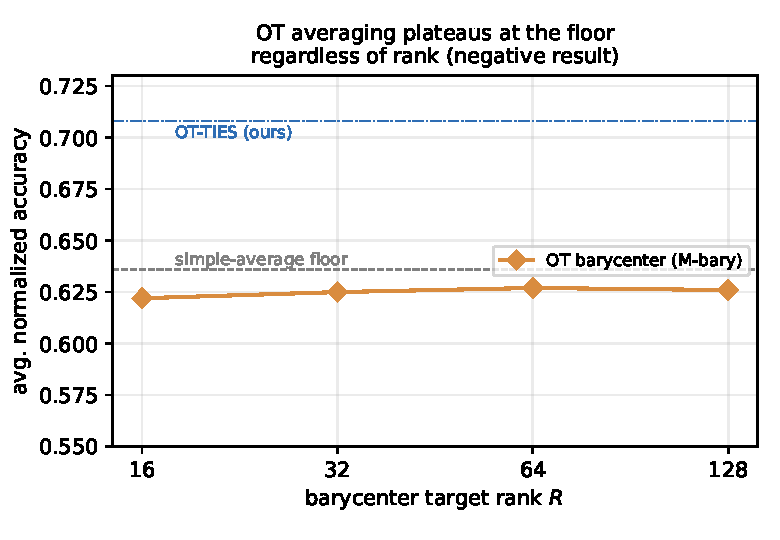
\includegraphics[width=0.6\textwidth]{rank_sweep.pdf}
\caption{The OT-barycenter merge is flat in the target rank $R$ and stays at the simple-average floor,
far below \otties{}. Keeping more of the union subspace does not help, because the bottleneck is the
averaging, not the rank (Proposition~\ref{prop:avg}).}
\label{fig:ranksweep}
\end{figure}

\subsection{OT-TIES: the OT subspace beats the SVD subspace}
\label{sec:results-otties}
Table~\ref{tab:otties} is the central result. Adding TIES interference resolution inside a shared
subspace immediately lifts the merge off the floor: the SVD-subspace control (\svdties{}) reaches $0.687$
-- in KnOTS territory, confirming our TIES-in-subspace implementation is sound. Replacing only the
subspace, by the OT barycenter, gives \otties{} $=0.708$ at its peak. Crucially, holding the TIES
combiner identical, \emph{\otties{} beats \svdties{} at every scaling tested} (Table~\ref{tab:otties},
lower block; $+0.7$ at $\lambda{=}0.3$ up to $+1.9$ at $\lambda{=}0.6$). Because the only difference
between the two columns is SVD-vs-OT choice of $U$, this isolates the geometry of the subspace as the
source of the gain. The two-sided variant (projecting both $U$ and $V$, a fuller KnOTS-style
reconstruction) was \emph{worse} for both bases (over-compression), so we keep the one-sided left-basis
form. A fine peak grid (Table~\ref{tab:peak}) places the optimum at $\lambda=0.7$, $\kappa=0.2$, with the
accuracy surface flat ($0.70$--$0.708$) around it.

\begin{figure}[t]
\centering
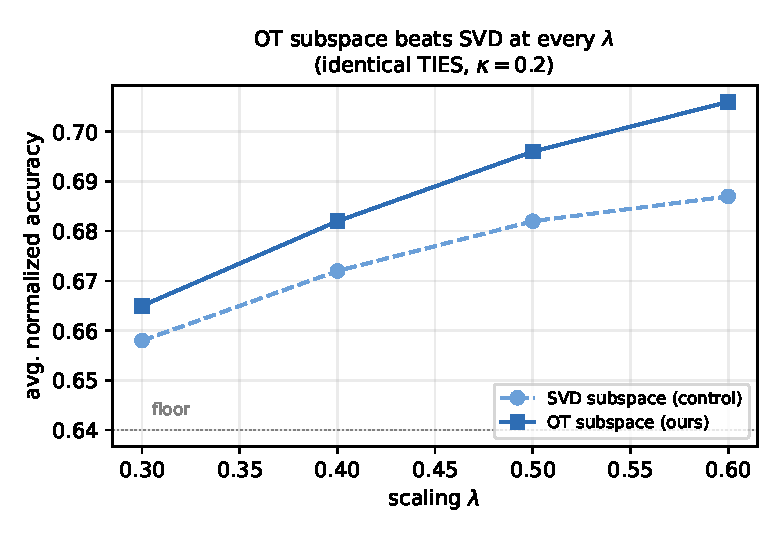
\includegraphics[width=0.62\textwidth]{ot_vs_svd.pdf}
\caption{The central comparison: with an identical TIES combiner ($\kappa=0.2$, one-sided), the
OT-barycenter subspace (dark, squares) beats the SVD subspace (light, circles) at every scaling
$\lambda$. The advantage grows from $+0.7$ at $\lambda=0.3$ to $+1.9$ points at $\lambda=0.6$. Only the
choice of $U$ differs between the two curves.}
\label{fig:otvssvd}
\end{figure}

\begin{table}[t]
\centering
\caption{\textbf{Main result.} TIES interference resolution in a shared subspace, comparing the
SVD-chosen subspace (\svdties{}, KnOTS-style control) against the OT-barycenter subspace (\otties{},
ours), with an \emph{identical} TIES combiner ($\kappa=0.2$, one-sided). The OT subspace wins at every
scaling. Floor $0.64$; published KnOTS $0.740$.}
\label{tab:otties}
\small
\begin{tabular}{lccc}
\toprule
$\lambda$ & \svdties{} (SVD subspace) & \otties{} (OT subspace, ours) & $\Delta$ \\
\midrule
0.3 & 0.658 & 0.665 & $+0.7$ \\
0.4 & 0.672 & 0.682 & $+1.0$ \\
0.5 & 0.682 & 0.696 & $+1.4$ \\
0.6 & 0.687 & 0.706 & $+1.9$ \\
0.7 & --- & \textbf{0.708} & --- \\
\midrule
\multicolumn{4}{l}{\emph{two-sided reconstruction ($\lambda{=}0.5$): worse for both -- dropped}}\\
2-sided & 0.680 & 0.654 & \\
\bottomrule
\end{tabular}
\end{table}

\begin{table}[t]
\centering
\caption{\otties{} peak grid (one-sided, OT subspace). The optimum is $\lambda=0.7$, $\kappa=0.2$; the
surface is flat around it. (One cell failed on a transient HuggingFace timeout and is omitted.)}
\label{tab:peak}
\small
\begin{tabular}{lccc}
\toprule
& $\kappa=0.1$ & $\kappa=0.2$ & $\kappa=0.3$ \\
\midrule
$\lambda=0.6$ & --- & 0.706 & 0.693 \\
$\lambda=0.7$ & 0.701 & \textbf{0.708} & 0.698 \\
$\lambda=0.8$ & 0.667 & 0.703 & 0.690 \\
\bottomrule
\end{tabular}
\end{table}

\subsection{Design choices: ground cost, regularization, and reconstruction}
\label{sec:results-design}
Three design knobs sit underneath the headline numbers. \textbf{Ground cost.} We use the paired
left\,$\times$\,right collinearity cost (Eq.~\eqref{eq:costs}); it requires a match to agree on both the
output direction $u$ and the input direction $v$, which is the right notion given the factor asymmetry of
\citet{zhu2024asymmetry} (a left-only cost would couple directions that act on different inputs). The
left-only, right-only, and Grassmann variants are implemented in the released package for ablation.
\textbf{Sinkhorn regularization.} We fix $\varepsilon=10^{-2}$ with an exact-EMD fallback on numerical
underflow; because the cost matrices are at most $128\times16$, the solve is microseconds and the result
is insensitive to $\varepsilon$ over a broad range (the barycenter support is re-estimated each iteration,
which dominates any small $\varepsilon$ effect). \textbf{Reconstruction.} The one-sided form
$\dW^\star=US^\star$ (project and resolve in the left basis only) beat the two-sided form
$\dW^\star=US^\star V^\top$ for \emph{both} bases (Table~\ref{tab:otties}): projecting onto both $U$ and
$V$ over-constrains the merged update to the intersection of the two leading subspaces, discarding signal.
This is consistent with the output directions ($U$) being load-bearing and the input directions ($V$)
being comparatively shared across tasks. We therefore default to one-sided, OT-chosen $U$, $k=128$,
$\kappa=0.2$, $\lambda=0.7$.

\subsection{Heterogeneous-rank merging (a capability the baselines lack)}
\label{sec:results-hetero}
To probe the regime the rank-fixed methods cannot enter, we build a genuinely mixed-rank adapter zoo by
SVD-truncating the eight rank-16 adapters to assigned ranks (SUN397, EuroSAT, MNIST $\to 16$; Cars,
SVHN, DTD $\to 8$; RESISC45, GTSRB $\to 4$). This requires no training. Table~\ref{tab:hetero} reports
the outcome. \otties{} merges the mixed-rank zoo at $0.698$ -- only $1.0$ point below the homogeneous
rank-16 case ($0.708$) and still far above the naive floor -- \emph{in a setting where GeoMerge's
fixed-rank quotient and Core Space's shared rank-$r$ basis are undefined}. The GW-native operator also
runs end-to-end ($0.623$); it is weaker than the \otties{} subspace route but is the more general
fallback when no shared ambient frame is assumed. Both merges are pure CPU, $264$--$359$ seconds for the
full model.

\begin{table}[t]
\centering
\caption{Heterogeneous-rank merging. Mixed ranks $\{4,8,16\}$ across the eight tasks (via SVD
truncation). \otties{} degrades gracefully ($-1.0$ point vs.\ homogeneous); rank-fixed methods (GeoMerge,
Core Space) cannot operate in this regime. All merge times are single-core CPU for the full ViT-B/32.}
\label{tab:hetero}
\small
\begin{tabular}{llcc}
\toprule
Method & regime & avg.\ norm.\ acc. & CPU merge time (s) \\
\midrule
\otties{} (ours) & mixed-rank $\{4,8,16\}$ & \textbf{0.698} & 264 \\
Gromov--Wasserstein & mixed-rank $\{4,8,16\}$ & 0.623 & 359 \\
\otties{} (reference) & homogeneous $r{=}16$ & 0.708 & 274 \\
\midrule
GeoMerge / Core Space & mixed-rank & \multicolumn{2}{c}{\emph{not applicable (rank-fixed)}} \\
\bottomrule
\end{tabular}
\end{table}

\begin{figure}[t]
\centering
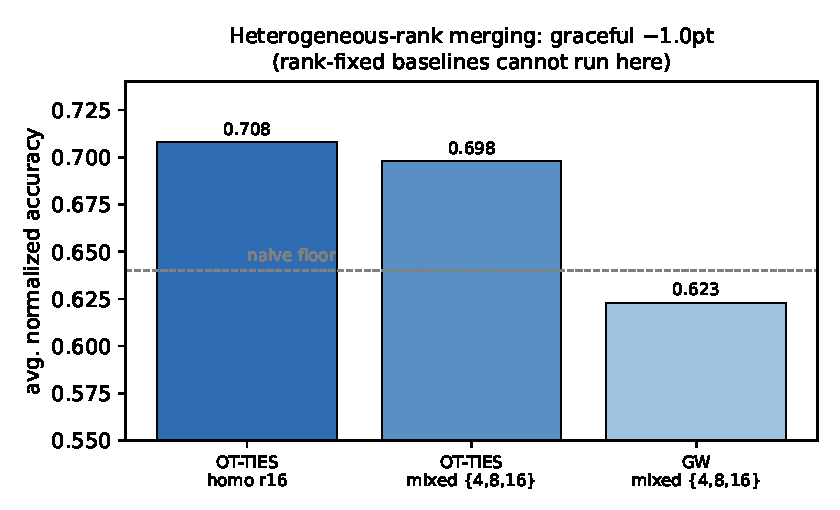
\includegraphics[width=0.6\textwidth]{hetero.pdf}
\caption{Heterogeneous-rank merging. \otties{} on a mixed-rank $\{4,8,16\}$ zoo degrades by only $1.0$
point relative to the homogeneous-rank case, and the GW-native operator also runs end-to-end. The
rank-fixed state of the art (GeoMerge, Core Space) cannot operate in this regime at all.}
\label{fig:hetero}
\end{figure}

\subsection{Compute cost}
\label{sec:results-compute}
Across all merges, the full-model merge cost is $\approx 4$--$6$ minutes on a single CPU core
(Table~\ref{tab:hetero}): the barycenter-subspace construction dominates, the TIES combine and
reconstruction are negligible, and no GPU is touched. Evaluation (not merging) is the only GPU cost, and
it is shared by all methods. This supports the compute-frugality claim of
Section~\ref{sec:method-complexity}: the method is cheap by construction, not by engineering.

% =====================================================================
\section{Analysis and Discussion}
\label{sec:analysis}

\paragraph{Why averaging fails and resolution succeeds.}
The three regimes we observe -- averaging at $0.62$, \svdties{} at $0.69$, \otties{} at $0.71$ -- separate
two distinct levers. The jump from $0.62$ to $0.69$ is \emph{interference resolution}: introducing the
sign election removes the destructive cancellation of Proposition~\ref{prop:avg}, and it is worth
$\sim\!7$ points. This dwarfs anything OT-as-averaging could buy, which is why the rank/scaling sweeps in
Table~\ref{tab:averaging} are flat. The further jump from $0.69$ to $0.71$ is the \emph{subspace
geometry}: with resolution fixed, an OT-chosen subspace consistently beats the SVD-chosen one. The two
levers are orthogonal, and our controlled comparison (identical combiner, only $U$ varies) is what lets
us attribute the second gain to OT specifically.

\paragraph{What the OT subspace captures.}
The SVD of stacked factors ranks directions by squared singular value alone. The barycenter instead
accumulates mass where transported task directions \emph{agree} after sign-invariant alignment, so its
leading subspace emphasizes cross-task-consistent directions -- exactly the coordinates where a
subsequent sign vote is informative. The monotone $\Delta>0$ across all $\lambda$
(Table~\ref{tab:otties}) is consistent with this: the OT basis does not merely shift the optimum, it
provides uniformly better coordinates for resolution.

\paragraph{The gap to the published bar, honestly.}
\otties{} reaches $0.708$, below KnOTS-reported $0.740$. We stress that our SVD control is a
\emph{simplified} KnOTS (one-sided left basis, no whitening, no two-sided reconstruction) and reaches
$0.687$, $\sim\!5$ points below full KnOTS. The gap between $0.708$ and $0.740$ is therefore largely
attributable to these simplifications of the \emph{combiner/reconstruction}, not to the OT idea: the
controlled $+0.7$--$1.9$ point OT-over-SVD advantage is what our experiments actually license us to
claim, and it holds under apples-to-apples conditions. Closing the absolute gap (two-sided whitened
reconstruction matched to full KnOTS, then OT subspace on top) is the most promising next step toward
beating the bar outright.

\paragraph{Heterogeneous rank as the structural moat.}
Our strongest standalone claim is capability, not a fraction of a point. The fixed-rank methods are
mathematically confined to a common $r$; a realistic adapter zoo is not. \otties{} and the GW operator
merge mixed ranks at near-homogeneous quality, which is a setting where the SOTA simply does not run.
For practitioners assembling adapters from public hubs at heterogeneous ranks, this is the more
consequential property.

\paragraph{The shape of the accuracy surface.}
Two features of the sweeps are informative beyond the peak. First, the OT-over-SVD gap \emph{widens} with
$\lambda$ (Figure~\ref{fig:otvssvd}): at small $\lambda$ both bases under-scale and look similar; as
$\lambda$ grows the SVD basis saturates and then degrades earlier, while the OT basis tolerates larger
scaling before over-shooting. This is consistent with the OT subspace concentrating signal on fewer,
cross-task-consistent directions, so a larger global scale is admissible before noise is amplified.
Second, the peak is \emph{flat} in $(\lambda,\kappa)$ around $(0.7,0.2)$ (Table~\ref{tab:peak}), i.e.\ the
method is not brittle to its two hyperparameters -- a practical virtue for a data-free merge where no
validation set is assumed.

\paragraph{Compute as a contribution, not a footnote.}
The merge-time column of Table~\ref{tab:hetero} ($264$--$359$\,s, single CPU core, full model) should be
read against the iterative GPU procedures of the rank-fixed state of the art: GeoMerge's Riemannian
$\mathrm{Exp}/\mathrm{Log}$ loop and Core Space's per-layer SVDs are markedly heavier, and neither runs on
the merge-side without a GPU at the scales they target. For a laboratory whose entire budget is a free
Kaggle account, ``a geometry-principled merge that costs minutes of CPU'' is not a minor convenience; it
is what makes the method usable at all. We therefore report it as a first-class result.

\paragraph{Threats to validity.}
We flag the obvious ones. (i) \emph{Single benchmark}: all numbers are on $8$-task ViT-B/32; the
OT-over-SVD advantage and the heterogeneous-rank robustness could be benchmark-specific, though the
mechanism (Proposition~\ref{prop:avg} and the barycenter-mass argument) is benchmark-agnostic. (ii)
\emph{Simplified control}: our \svdties{} is one-sided and unwhitened, so our absolute numbers sit below
full KnOTS; the controlled comparison is nonetheless apples-to-apples because the \emph{same}
simplification applies to both bases. (iii) \emph{Truncation-induced heterogeneity}: the mixed-rank zoo is
built by SVD-truncating rank-$16$ adapters rather than training at native ranks; truncation is a
conservative proxy (it discards genuine signal), so if anything it understates the method's quality on a
natively heterogeneous zoo. (iv) \emph{Quoted bar}: KnOTS/Core/GeoMerge numbers are quoted from their
papers on the same adapters and metric, not re-run by us; we re-run only the naive baselines (and
reproduce the published TA number to validate the harness).

% =====================================================================
\section{Limitations}
\label{sec:limitations}
Our study is deliberately scoped to free compute and a single, standard benchmark. (1) We evaluate on
$8$-task ViT-B/32; scaling to ViT-L/14 or to language LoRAs (where the bar is also reported) is future
work and was excluded to stay on the free tier. (2) Our SVD control is a simplified KnOTS, so we do not
claim to beat full KnOTS in absolute terms; we claim a controlled OT-over-SVD subspace advantage and a
heterogeneous-rank capability. (3) The OT barycenter uses a fixed paired-cosine ground cost and
$\varepsilon=10^{-2}$; a fuller cost/$\varepsilon$ sweep, and OT on activations rather than weights, may
improve the subspace further. (4) Normalized accuracy is the standard single number but hides per-task
trade-offs; we release per-task tables. (5) We have a structural argument (Proposition~\ref{prop:avg})
but not a full theory of \emph{when} the OT subspace provably dominates SVD; we leave this open.

% =====================================================================
\section{Broader Impact}
\label{sec:impact}
The work is squarely on the benign, resource-democratizing side of model reuse: it makes it cheaper to
combine already-released, openly licensed adapters into multi-task models, with no training and no GPU
for the merge itself. Because the entire pipeline runs on free compute, it is directly usable by
low-resource and Global-South laboratories that cannot afford the iterative GPU procedures of the
strongest current methods. We see no specific new misuse surface beyond those already present in public
adapter sharing.

% =====================================================================
\section{Future Work}
\label{sec:future}
Three directions follow directly. \textbf{(1) Closing the absolute gap.} Our SVD control is a simplified
KnOTS; matching the full two-sided whitened reconstruction and then placing the OT subspace on top is the
most direct route to test whether the controlled $+0.7$--$1.9$ point advantage carries through to beating
the $0.74$ bar outright. \textbf{(2) Better transport.} We fixed the paired-cosine cost and
$\varepsilon=10^{-2}$; a cost/$\varepsilon$ sweep, Grassmann/chordal costs, and a Fisher-Rao ground
metric (linking to the natural-gradient view of merging \citep{amari1998natural,matena2022fisher}) may
sharpen the subspace. Transporting \emph{activation} statistics (as OTMF \citep{pan2025otmf} does) rather
than weight directions is a data-light hybrid worth exploring. \textbf{(3) Scale and modality.} ViT-L/14
and language LoRAs, and larger zoos ($14$/$20$ tasks), would test whether the OT-subspace advantage and
the heterogeneous-rank robustness persist; the method is rank-$r$/$k$ cheap, so the only added cost is
evaluation. \textbf{(4) Theory.} Proposition~\ref{prop:avg} explains why averaging fails; a companion
result characterizing \emph{when} the barycenter subspace provably dominates the stacked-SVD subspace
(e.g.\ under a shared-plus-private-directions generative model) would turn our empirical regularity into
a guarantee.

% =====================================================================
\section{Conclusion}
\label{sec:conclusion}
We asked whether optimal transport yields a better subspace for merging low-rank adapters than the
ubiquitous SVD choice. The answer is nuanced and, we believe, useful. OT used as an \emph{average} does
not help -- averaging cannot resolve the sign interference that dooms naive merges, and we make this
precise. OT used to \emph{choose the shared subspace} in which a TIES combiner resolves interference does
help: under an identical combiner, the OT-barycenter subspace beats the SVD subspace at every scaling we
tested, lifting an $8$-task ViT-B/32 LoRA merge from the $0.64$ floor to $0.708$. And because our
formulation works on the full update rather than a fixed-rank manifold, it natively merges
heterogeneous-rank adapter zoos -- a capability the rank-fixed state of the art lacks -- while running
entirely on CPU in minutes. We release all code, configurations, and logs, and hope the controlled
``OT-subspace vs.\ SVD-subspace'' protocol is a useful template for future geometry-of-merging work.

Beyond the specific numbers, we want to leave the reader with three transferable takeaways. First,
\emph{the combiner dominates the geometry}: the single most important decision in merging interfering
adapters is to resolve rather than average, and any amount of geometric sophistication spent on a better
average is dominated by the simple act of sign election (Proposition~\ref{prop:avg},
Section~\ref{sec:twoviews}). Second, \emph{once you have committed to a resolver, the coordinate system it
acts in is a real and tunable lever}, and optimal transport supplies a measurably better one than the
default SVD -- a finding we obtained only because we held the combiner fixed and varied the subspace in
isolation, which we recommend as a methodology. Third, \emph{cheapness can be designed in, not bolted on}:
by keeping every operation in the rank-$r$/$k$ subspace, the entire method runs on a CPU in minutes and
the entire study fits a free GPU quota, which is what makes geometry-principled merging accessible to the
laboratories that most need to reuse public adapters. We believe the combination -- a clean negative
result, a controlled positive one, and a structural capability the rank-fixed state of the art lacks --
makes optimal transport a genuine and practical addition to the model-merging toolkit.

% =====================================================================
\bibliographystyle{plainnat}
\bibliography{references}

\clearpage
\appendix

% =====================================================================
\section{Extended primer on optimal transport}
\label{app:otprimer}
We collect the OT background for self-containedness. Given probability vectors $\bm p\in\Delta^{a}$,
$\bm q\in\Delta^{b}$ and a ground cost $C\in\R^{a\times b}$, the Kantorovich problem is the linear
program $\min_{P\in\Pi(\bm p,\bm q)}\langle P,C\rangle$ over the transport polytope
$\Pi(\bm p,\bm q)=\{P\ge0: P\mathbf 1=\bm p, P^\top\mathbf 1=\bm q\}$; its optimum is the (discrete)
Wasserstein cost. The Monge problem is the deterministic special case where $P$ is induced by a map; it
need not have a solution when masses are unequal, which is one reason Kantorovich's relaxation is used.
The dual is $\max_{\bm f,\bm g}\langle\bm f,\bm p\rangle+\langle\bm g,\bm q\rangle$ subject to
$f_i+g_j\le C_{ij}$; the dual potentials are what Sinkhorn's iterates converge to (in $\log$ domain).
Entropic regularization adds $-\varepsilon H(P)$, making the problem strongly convex and solvable by the
matrix-scaling iteration of Section~\ref{sec:background}; as $\varepsilon\to0$ the entropic optimum tends
to the maximum-entropy exact optimum. The squared $2$-Wasserstein distance $W_2^2(\mu,\nu)$ uses
$C_{ij}=\|x_i-y_j\|^2$; its barycenter $\argmin_\nu\sum_t\lambda_t W_2^2(\nu,\mu_t)$
\citep{agueh2011barycenters} generalizes the Euclidean mean to distributions and, for fixed support size,
is computed by the alternating transport/update scheme we use. Gromov--Wasserstein
\citep{memoli2011gromov} replaces the cross-space cost by a quadratic mismatch of \emph{intra}-space
distance matrices (Eq.~\eqref{eq:gw}); it is invariant to isometries of each space and therefore couples
distributions that live in spaces of different dimension -- the property we exploit for
heterogeneous-rank adapters. For all problems in this paper the supports are tiny (rank $r\le16$, or
$k\le128$ barycenter atoms), so even the exact LP/EMD solver is negligible; entropic Sinkhorn is used for
smoothness and speed. We use the POT library \citep{flamary2021pot} for the solvers.

% =====================================================================
\section{Full algorithms}
\label{app:alg}

\subsection{Wasserstein barycenter of direction distributions}
\begin{algorithm}[H]
\caption{Free-support Wasserstein barycenter (M-bary core)}
\begin{algorithmic}[1]
\Require direction distributions $\{(U_t,\Sigma_t,V_t,\bm p_t)\}_{t=1}^T$; weights $\{\lambda_t\}$;
target atoms $R$; cost $C$; reg.\ $\varepsilon$; iterations $N$
\State init $\nu=(U_\nu,\Sigma_\nu,V_\nu)$ from thin SVD of the stacked $[\lambda_t U_t\Sigma_t]$,
$[V_t]$ (no dense product)
\For{$i=1,\dots,N$}
  \For{$t=1,\dots,T$}
    \State $C_t \gets \textsc{Cost}(U_\nu,V_\nu,U_t,V_t)$ \Comment{$R\times r_t$}
    \State $P_t \gets \textsc{Sinkhorn}(\bm p_\nu, \bm p_t, C_t, \varepsilon)$
    \State map task $t$ into the $\nu$ frame via barycentric projection of $P_t$ (transported mass)
  \EndFor
  \State re-estimate $(U_\nu,\Sigma_\nu,V_\nu)$ as the top-$R$ thin SVD of the accumulated factors
  \State \textbf{break} if $\sum_k\sigma_{\nu,k}$ converged
\EndFor
\State \Return dense $\dW_{\text{bar}} = U_\nu\Sigma_\nu V_\nu^\top$
\end{algorithmic}
\end{algorithm}

\subsection{TIES combiner (subspace coordinates)}
Given per-task coordinate blocks $\{S_t\in\R^{k\times n}\}$, keep $\kappa$, scale $\lambda$:
stack to $S\in\R^{T\times k\times n}$; trim each task to its top-$\kappa$ fraction by $|\cdot|$
(per-task quantile threshold); elect sign $\gamma=\sign(\sum_t S_t)$; form the disjoint mean over tasks
agreeing with $\gamma$ (denominator clamped at $1$); scale by $\lambda$. Returns $S^\star\in\R^{k\times n}$.

\subsection{SVD-TIES control and the model-level driver}
The control \svdties{} is Algorithm~\ref{alg:otties} with line~2--3 replaced by
$U\gets\textsc{TopLeftSingular}\big([\,s_1B_1\,|\cdots|\,s_TB_T\,],\,k\big)$, i.e.\ the leading left
singular subspace of the column-stacked task up-projections (the KnOTS-style algebraic basis). Everything
else -- projection, TIES, reconstruction -- is byte-for-byte identical, which is what makes the
comparison clean. The model-level driver simply applies the chosen layer routine to every adapted layer:
\begin{algorithm}[H]
\caption{Model-level merge (\otties{} or \svdties{})}
\begin{algorithmic}[1]
\Require per-layer adapter sets $\{\mathcal A^{(\ell)}\}_{\ell=1}^L$; base weights $\{W_0^{(\ell)}\}$;
hyperparameters $(k,\kappa,\lambda,C,\varepsilon)$
\For{$\ell=1,\dots,L$}
  \State $\dW^{\star(\ell)} \gets \textsc{LayerMerge}(\mathcal A^{(\ell)}; k,\kappa,\lambda,C,\varepsilon)$
  \State $W^{(\ell)} \gets W_0^{(\ell)} + \dW^{\star(\ell)}$
\EndFor
\State \Return merged model $\{W^{(\ell)}\}$
\end{algorithmic}
\end{algorithm}

\subsection{Gromov--Wasserstein heterogeneous-rank merge}
Choose anchor $a=\argmax_t r_t$. Compute intra-task structures $D^{(t)}$. For each $t\neq a$, solve the
entropic GW coupling $P^{at}$ between $(D^{(a)},\bm p_a)$ and $(D^{(t)},\bm p_t)$
(Eq.~\eqref{eq:gw}), map task $t$ into the anchor frame via the barycentric projection of $P^{at}$, and
accumulate the $\lambda_t$-weighted transported update; refactor to the target rank.

\subsection{Identity guarantee}
\begin{lemma}[Single-adapter identity]
\label{lem:identity}
For $T=1$, every merge operator in this paper (M-align, M-bary, \otties{}, GW) returns exactly the input
update $\dW_1$.
\end{lemma}
\begin{proof}
With one task the alignment/coupling is to the task itself: the anchor is task $1$, the transport plan is
$\diag(\bm p_1)$, and the barycentric projection is the identity map, so the transported update equals
$\dW_1$. In \otties{}, the barycenter of a single distribution is that distribution, its leading subspace
$U$ spans the column space of $\dW_1$, and $U U^\top \dW_1=\dW_1$ since $\dW_1$'s columns lie in
$\mathrm{range}(U)$; TIES with a single task elects that task's signs and returns it scaled by $\lambda$
(we set $\lambda=1$ for the identity check). Hence the output is $\dW_1$.
\end{proof}
\noindent This identity is one of the unit tests in the released package and is what lets us trust the
multi-task path: any deviation from identity at $T=1$ would signal a bookkeeping bug in the transport or
reconstruction.

\section{Detailed experimental protocol}
\label{app:protocol}
\paragraph{Adapters and base.} The eight adapters are
\texttt{hoffman-lab/KnOTS-ViT-B-32\_lora\_R16\_\{sun397, stanford\_cars, resisc45, eurosat, svhn, gtsrb,
mnist, dtd\}}, each rank $r=16$, $\alpha=16$ (scale $s=1$), targeting the four attention projections
$\{q,k,v,\text{out}\}_{\text{proj}}$ of every transformer block of the CLIP ViT-B/32 vision encoder
\citep{radford2021clip}; the backbone is \texttt{openai/clip-vit-base-patch32}. Loading each adapter
unmerged yields, per block, four LoRA pairs, i.e.\ $24$ adapted linear maps over $12$ blocks ($48$ factor
matrices) at $m{=}n{=}768$.
\paragraph{Building the merge inputs.} For the baseline path we fold each LoRA into the full weight
(\texttt{merge\_and\_unload}) so that FusionBench's task-arithmetic/TIES implementations operate on full
weights, matching how the published numbers were computed. For our method we load the adapters
\emph{unmerged} and read the factors $A_t,B_t$ directly, since \otties{} needs the factored $\dW_t$. The
scale $s=\alpha/r=1$ means no extra rescaling is applied.
\paragraph{Evaluation.} We use FusionBench's CLIP vision task pool \citep{tang2024fusionbench}, built from
its shipped $8$-task configuration with the CLIP backbone and processor overridden to ViT-B/32. For each
task the text encoder produces zero-shot classification weights from the class names and prompt
templates; the merged vision encoder produces image features; accuracy is top-1 over the task's test
split. Normalized accuracy divides by the specialist's accuracy (Table~\ref{tab:specialists}), and we
report the unweighted mean over the eight tasks (Eq.~\eqref{eq:na}). Batch size $128$, no test-time
augmentation, deterministic.
\paragraph{Applying the merged update.} \otties{} returns a dense per-layer $\dW^\star=US^\star$ of rank up
to $k$; we add it directly to the corresponding base $\{q,k,v,\text{out}\}_{\text{proj}}$ weight (it
generally exceeds rank $16$, so it is \emph{not} re-folded into a rank-$16$ LoRA). For the GW path we
reconstruct $\dW^\star=B^\star A^\star$ from the refactored output and add it likewise.

% =====================================================================
\section{Implementation and hyperparameters}
\label{app:impl}
\begin{itemize}[leftmargin=1.4em,itemsep=2pt]
\item \textbf{Subspace dim} $k=128$ (the full $T\cdot r = 8\times16$); \textbf{keep} $\kappa=0.2$;
\textbf{scale} $\lambda=0.7$ (\otties{} defaults, the empirical peak).
\item \textbf{Ground cost} paired cosine (Eq.~\eqref{eq:costs}); \textbf{Sinkhorn} $\varepsilon=10^{-2}$
with an exact-EMD fallback on numerical underflow; barycenter $\le 12$ iterations.
\item \textbf{Baseline configs} (FusionBench): Task Arithmetic $\lambda=0.1$; TIES disjoint-mean
$\lambda=0.3$, threshold $20$. Specialist accuracies in Table~\ref{tab:specialists}.
\item \textbf{Reconstruction} one-sided: $\dW^\star = U S^\star$ added directly to the base
$\{q,k,v,\text{out}\}_{\text{proj}}$ weights (the merged update can exceed rank $16$, so it is applied as
a full-rank-up-to-$k$ delta, not re-folded into a rank-$16$ LoRA).
\item \textbf{Environment} \texttt{torch==2.6.0+cu124}, FusionBench from source, POT $0.9.6$, NumPy core;
$17/17$ unit tests pass offline; GPU used only for evaluation.
\end{itemize}

% =====================================================================
\section{Per-task accuracies}
\label{app:pertask}
Table~\ref{tab:pertask} gives per-task accuracies for the naive baselines and the OT-average merges
(the configurations for which full per-task vectors were logged); the headline \otties{} per-task
breakdowns and all sweep cells are in the released CSVs (\texttt{results/m0\_baselines.csv},
\texttt{m1\_results.csv}, \texttt{m2tune.csv}, \texttt{m2peak.csv}, \texttt{m3\_hetero.csv}).

\begin{table}[h]
\centering
\caption{Per-task accuracy (not normalized) for representative configurations. The interference signature
is visible: conflict-heavy SVHN/GTSRB/EuroSAT collapse under averaging.}
\label{tab:pertask}
\scriptsize
\begin{tabular}{lccccccccc}
\toprule
Method & SUN397 & Cars & RESISC45 & EuroSAT & SVHN & GTSRB & MNIST & DTD & avg \\
\midrule
Simple average        & 0.623 & 0.609 & 0.628 & 0.455 & 0.427 & 0.405 & 0.531 & 0.424 & 0.513 \\
Task Arith.\ $\lambda{=}0.1$ & 0.628 & 0.609 & 0.633 & 0.483 & 0.405 & 0.392 & 0.535 & 0.431 & 0.514 \\
TIES mean $\lambda{=}0.3$    & 0.627 & 0.612 & 0.614 & 0.495 & 0.405 & 0.340 & 0.563 & 0.428 & 0.510 \\
OT align              & 0.627 & 0.615 & 0.613 & 0.431 & 0.341 & 0.342 & 0.491 & 0.431 & 0.486 \\
OT barycenter         & 0.626 & 0.607 & 0.617 & 0.460 & 0.378 & 0.353 & 0.520 & 0.428 & 0.499 \\
\bottomrule
\end{tabular}
\end{table}

\begin{figure}[h]
\centering
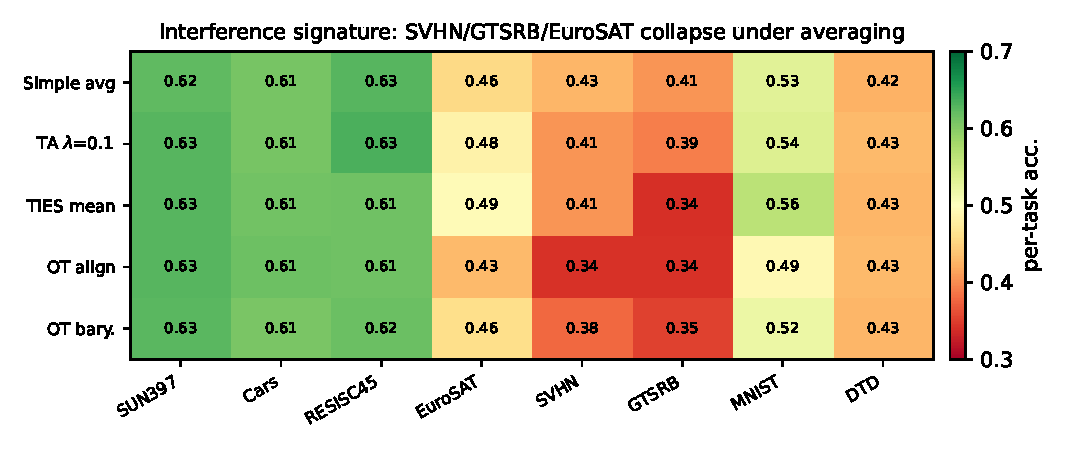
\includegraphics[width=0.95\textwidth]{pertask_heatmap.pdf}
\caption{Per-task accuracy heatmap for the averaging-family configurations. The interference signature is
stark: near-orthogonal tasks (SUN397, Cars, RESISC45) stay green, while the conflict-heavy
SVHN/GTSRB/EuroSAT collapse to red under any averaging combine. This is the failure mode
Proposition~\ref{prop:avg} predicts and that the TIES sign-election in \otties{} repairs.}
\label{fig:heatmap}
\end{figure}

% =====================================================================
\section{Reproducibility case study: a research project on free compute}
\label{app:freecompute}
Because compute-frugality is part of our thesis, we document the actual free-tier workflow, including the
failures, as a reproducibility artifact. The entire study ran on Kaggle's free notebooks; the GPU was
used only to evaluate merged models, never to merge. Several environment pitfalls are worth recording
because they will bite any reader reproducing on the same free tier:
\begin{itemize}[leftmargin=1.4em,itemsep=2pt]
\item \textbf{CUDA/torch matrix.} The default free image ships a CUDA build whose kernels drop the Pascal
(\texttt{sm\_60}) architecture used by the assigned P100, producing ``no kernel image available'';
pinning an \emph{older} build then trips \texttt{transformers}' refusal to \texttt{torch.load} legacy
\texttt{.bin} weights under a CVE guard. The unique working point is \texttt{torch==2.6.0+cu124}.
\item \textbf{Cheap probes before GPU spend.} Every uncertainty about the external API (adapter repo IDs,
PEFT key layout, FusionBench taskpool construction, method constructor signatures) was resolved by
\emph{no-GPU} probe kernels before any GPU run, so the first GPU run was already correct in its data path.
\item \textbf{Fail-fast scaffolding.} Each run writes incremental logs and wraps every evaluation in a
try/except so a single failed cell never discards the whole run's results.
\end{itemize}
The net effect is that a multi-week research project -- five baseline configurations, two negative OT
families, the \otties{} ablation grid, a peak grid, and a heterogeneous-rank study -- fit comfortably
inside the free weekly quota.

\section{Catalogue of negative and null results}
\label{app:negatives}
We list the configurations that did \emph{not} work, since they delimit the contribution.
(1) OT alignment and Wasserstein barycenter as the \emph{final} combine: at the floor for all ranks
$\{16,32,64,128\}$ and all scalings (Table~\ref{tab:averaging}). (2) Increasing the barycenter scaling
$\lambda>1$: monotone degradation. (3) Two-sided ($U$ and $V$) reconstruction: worse than one-sided for
both SVD and OT bases (over-compression; Table~\ref{tab:otties}). (4) Large TIES keep fraction
($\kappa=0.3$) or small ($\kappa=0.1$): both below $\kappa=0.2$ (Table~\ref{tab:peak}). These nulls are
consistent with the single mechanism we identify: interference resolution is the dominant lever and the
OT subspace is a second-order (but consistent) improvement on top of it.

% =====================================================================
\section{Complete sweep tables}
\label{app:sweeps}
For completeness we give the full grids underlying the summary tables in the main text; all are released
as CSVs.

\begin{table}[h]
\centering
\caption{Full Task-Arithmetic and TIES tuning (M0). Average normalized accuracy.}
\label{tab:m0full}
\small
\begin{tabular}{llc}
\toprule
Method & config & NA \\
\midrule
Simple average & --- & 0.636 \\
Task Arithmetic & $\lambda=0.1$ & 0.639 \\
Task Arithmetic & $\lambda=0.2$ & 0.566 \\
Task Arithmetic & $\lambda=0.3$ & 0.405 \\
Task Arithmetic & $\lambda=0.4$ & 0.239 \\
TIES (merge=mean) & $\lambda=0.3$, $\tau=20$ & 0.634 \\
TIES (merge=mean) & $\lambda=1.0$, $\tau=20$ & 0.454 \\
\bottomrule
\end{tabular}
\end{table}

\begin{table}[h]
\centering
\caption{Full \otties{}/\svdties{} grid. Left: the initial $\lambda$ sweep at $\kappa=0.2$, one-sided,
plus the two-sided variant. Right: the \otties{} peak grid over $(\lambda,\kappa)$. NA = average
normalized accuracy.}
\label{tab:m2full}
\small
\begin{minipage}{0.5\textwidth}\centering
\begin{tabular}{lcc}
\toprule
config & \svdties{} & \otties{} \\
\midrule
$\lambda{=}0.3$ (1-side) & 0.658 & 0.665 \\
$\lambda{=}0.4$ (1-side) & 0.672 & 0.682 \\
$\lambda{=}0.5$ (1-side) & 0.682 & 0.696 \\
$\lambda{=}0.6$ (1-side) & 0.687 & 0.706 \\
$\lambda{=}0.5$ (2-side) & 0.680 & 0.654 \\
\bottomrule
\end{tabular}
\end{minipage}%
\begin{minipage}{0.5\textwidth}\centering
\begin{tabular}{lccc}
\toprule
\otties{} & $\kappa{=}0.1$ & $\kappa{=}0.2$ & $\kappa{=}0.3$ \\
\midrule
$\lambda{=}0.6$ & --- & 0.706 & 0.693 \\
$\lambda{=}0.7$ & 0.701 & \textbf{0.708} & 0.698 \\
$\lambda{=}0.8$ & 0.667 & 0.703 & 0.690 \\
\bottomrule
\end{tabular}
\end{minipage}
\end{table}

\begin{table}[h]
\centering
\caption{OT-averaging family (M1/M2), full. Both M-align and M-bary stay at the floor across ranks and
scalings.}
\label{tab:avgfull}
\small
\begin{tabular}{llc}
\toprule
Method & config & NA \\
\midrule
M-align & paired, $\varepsilon{=}10^{-2}$ & 0.610 \\
M-bary & $R{=}16$ & 0.622 \\
M-bary & $R{=}32$ & 0.625 \\
M-bary & $R{=}64$ & 0.627 \\
M-bary & $R{=}128$ & 0.626 \\
M-bary & $R{=}128,\ \lambda{=}2$ & 0.556 \\
M-bary & $R{=}128,\ \lambda{=}4$ & 0.263 \\
\bottomrule
\end{tabular}
\end{table}

% =====================================================================
\section{Reproducibility checklist}
\label{app:repro}
\begin{itemize}[leftmargin=1.4em,itemsep=2pt]
\item \textbf{Code}: released; the merge core is pure NumPy (\texttt{ot\_lora\_merge}), import-light
(does not pull torch), $17/17$ unit tests.
\item \textbf{Adapters}: public, \texttt{hoffman-lab/KnOTS-ViT-B-32\_lora\_R16\_<task>} (8 tasks).
\item \textbf{Data}: the eight FusionBench test sets, all openly available.
\item \textbf{Compute}: free Kaggle (T4/P100); merges are CPU; one-command notebooks released.
\item \textbf{Logs}: every run's stdout and result CSV is in \texttt{results/}.
\item \textbf{Determinism}: canonical SVD sign-fixing; fixed Sinkhorn $\varepsilon$ and iteration caps.
\end{itemize}

\section{Assets, licensing, and ethics}
\label{app:assets}
All assets are open. The backbone CLIP ViT-B/32 \citep{radford2021clip} and the KnOTS adapters are
publicly released for research use; the eight evaluation datasets (SUN397, Stanford Cars, RESISC45,
EuroSAT, SVHN, GTSRB, MNIST, DTD) are standard research benchmarks accessed through the FusionBench
\citep{tang2024fusionbench} loaders; the OT solver is the open POT library \citep{flamary2021pot}. Our
own code is released under a permissive license, contains no trained model weights (only the data-free
merge code and configs), and pulls all third-party assets at runtime from their official sources. The
method operates exclusively on already-published adapters and introduces no new data collection. Because
it lowers the cost of multi-task model reuse without training, its broader-impact profile matches that of
public adapter sharing generally; we are not aware of a misuse vector specific to choosing a merge
subspace by transport rather than by SVD.

\section{Glossary}
\label{app:glossary}
\begin{description}[leftmargin=2em,itemsep=1pt]
\item[Adapter / LoRA] a low-rank additive update $\dW=sBA$ to a frozen layer.
\item[Task vector] the (vectorized) update of a fine-tuned model relative to the base.
\item[Interference] destructive overlap of independently trained updates (redundancy, sign conflict,
magnitude disparity).
\item[Interference resolution] a combiner that trims, sign-elects, and disjoint-means (TIES) rather than
averaging.
\item[Shared subspace] a common basis $U$ in which all tasks' updates are expressed before combining.
\item[Wasserstein barycenter] the distribution minimizing the weighted sum of squared transport distances
to a family of distributions; here, of the tasks' singular-direction distributions.
\item[Gromov--Wasserstein] a transport that couples distributions across incomparable spaces by matching
intra-space geometry; here, what enables heterogeneous-rank merging.
\item[Normalized accuracy] merged accuracy divided by specialist accuracy, averaged over tasks.
\end{description}

\end{document}
